\documentclass[11pt,a4paper,oneside]{report}

\usepackage{graphicx} % En­hanced sup­port for graph­ics
\graphicspath{ {./images/} }

\usepackage[tmargin=1in,bmargin=1in,lmargin=1.38in,rmargin=0.79in]{geometry} % Set margin size for document (same as Microsoft Normal margins)

\usepackage{times} % Select Adobe Times Ro­man (or equiv­a­lent) as de­fault font
\usepackage{epsfig} % In­clude En­cap­su­lated PostScript in LaTeX doc­u­ment
\usepackage{fancyhdr} % Ex­ten­sive con­trol of page head­ers and foot­ers
\usepackage{longtable} % Al­low ta­bles to flow over page bound­aries
\usepackage{subfig} % Ma­nip­u­la­tion and ref­er­ence of small subfigures
\usepackage{color} % Colour con­trol
\usepackage{amsmath} % Mathematical typsetting
\usepackage{amssymb} % Provides an extended symbol collection
\usepackage{bm} % Bold sym­bols in maths mode
\usepackage{psfrag} % For proper math symbols in postscript plots
\usepackage{url} % Allow for URL to be entered
\usepackage[linktocpage]{hyperref} % Ex­ten­sive sup­port for hy­per­text

\usepackage[square,numbers]{natbib} % Bibliography

\definecolor{ashgrey}{rgb}{0.7, 0.75, 0.71}


\usepackage{setspace} % Allow for custom setting space be­tween lines

\usepackage{multicol} % In­ter­mix sin­gle and mul­ti­ple columns
\usepackage{paralist} % Enu­mer­ate and item­ize within para­graphs
\usepackage{floatrow} % Mod­i­fy­ing the lay­out of floats

%\setlength{\parindent}{0pt} % Remove paragraph indent
\setlength{\parskip}{\baselineskip} % Force skip line between paragraphs
\floatsetup[table]{capposition=top} % Position caption on top of tables


%%% Setting the Chapter and Section settings to Surrey requirements %%%
\usepackage{titlesec}
\titleformat{\chapter}[block]
{\fontsize{12}{15}\bfseries}
{\thechapter}
{1em}
{\MakeUppercase}
\titlespacing*{\chapter}{0pt}{1pt}{0pt}[0pt]

\titleformat{\section}[block]
{\fontsize{12}{15}\bfseries}
{\thesection}
{1em}
{}
\titlespacing*{\section}{0pt}{0pt}{-12pt}[0pt]

\titleformat{\subsection}[block]
{\fontsize{12}{15}\bfseries}
{\thesubsection}
{1em}
{}
\titlespacing*{\subsection}{0pt}{0pt}{-12pt}[0pt]

\titleformat{\subsubsection}[block]
{\fontsize{12}{15}}
{\thesubsubsection}
{1em}
{}
\titlespacing*{\subsubsection}{0pt}{0pt}{-12pt}[0pt]
%%%%%%

\newcommand{\squeezeup}{\vspace{-2.5mm}} % Reduce spacing manually
\clubpenalty = 10000 % eliminates orphans
\widowpenalty = 10000 % eliminates orphans


\usepackage{style/myfootnote} % footnote settings
\makesavenoteenv{longtable}
\usepackage{vmargin}
\input{./style/epsf.sty}

%%%%%%%%%%%%%%%%%%%%%%%%%%%%%%%%%%%%%%%%%%%%%%%%%%%%%%%%%%%%%%%%%%%%
%%%%%%%%%%%%%%%%%%%%%%%%%%%%%%%%%%%%%%%%%%%%%%%%%%%%%%%%%%%%%%%%%%%%
%        parameters used for page setup and figure placement
%%%%%%%%%%%%%%%%%%%%%%%%%%%%%%%%%%%%%%%%%%%%%%%%%%%%%%%%%%%%%%%%%%%%
%%%%%%%%%%%%%%%%%%%%%%%%%%%%%%%%%%%%%%%%%%%%%%%%%%%%%%%%%%%%%%%%%%%%


%line spacing
\setstretch{1.5}%1.}

%%%%%%%%%%%%%%%%%%%%%%%%%%%%%%%%%%%%%%%%%%%%%%%%%%%%%%%%%%%%%%%%%%%%
% change the allowed picture fractions
%%%%%%%%%%%%%%%%%%%%%%%%%%%%%%%%%%%%%%%%%%%%%%%%%%%%%%%%%%%%%%%%%%%%
\renewcommand{\textfraction}{0.15}
\renewcommand{\topfraction}{0.9}
\renewcommand{\bottomfraction}{0.65}
\renewcommand{\floatpagefraction}{0.6}


%%%%%%%%%%%%%%%%%%%%%%%%%%%%%%%%%%%%%%%%%%%%%%%%%%%%%%%%%%%%%%%%%%%%
% set page dimensions
%%%%%%%%%%%%%%%%%%%%%%%%%%%%%%%%%%%%%%%%%%%%%%%%%%%%%%%%%%%%%%%%%%%%
%put \hoffset = -1in then \oddsidemargin = left margin
%put \voffset = -1in then \topmargin = top margin


%\setmargins{leftmargin}{topmargin}{textwidth}{textheight}{headheight}...
%       {headsep}{footheight}{footskip}
%\setmargins{25mm}{15mm}{160mm}{250mm}{7mm}{7mm}{0pt}{10mm}
\setmargins{40mm}{20mm}{150mm}{235mm}{7mm}{7mm}{0pt}{8mm}
%6.5in15

% DARACH's
%\setlength{\hoffset}{-1.5in}%-1in}
%\setlength{\voffset}{-1.5in}%-1in}
%\setlength{\topmargin}{1.0in}%25in}
%\setlength{\oddsidemargin}{1.5in}
%\setlength{\textwidth}{6.25in}%5.75in}
%\setlength{\textheight}{9.9in}%8.33in}
%\setlength{\headheight}{8pt}%12pt}
%\setlength{\headsep}{20pt}
%\setlength{\footskip}{30pt}%48pt}

%%%%%%%%%%%%%%%%%%%%%%%%%%%%%%%%%%%%%%%%%%%%%%%%%%%%%%%%%%%%%%%%%%%%
%       page header
%%%%%%%%%%%%%%%%%%%%%%%%%%%%%%%%%%%%%%%%%%%%%%%%%%%%%%%%%%%%%%%%%%%%


\pagestyle{fancyplain}
%\renewcommand{\chaptermark}[1]{\markboth{#1}{}}
%\renewcommand{\sectionmark}[1]{\markright{\thesection\ #1}}
\renewcommand{\subsectionmark}[1]{\markright{\thesubsection\ #1}}
\rhead{\fancyplain{}{\bfseries\rightmark}} \lhead{}
    \lhead{}  % TO ADD THE DATE TO THE HEADING, need entry even if empty
    %\lhead{\today}  % TO ADD THE DATE TO THE HEADING, need entry even if empty
\addtocounter{secnumdepth}{1} \addtocounter{tocdepth}{1}


%%%%%%%%%%%%%%%%%%%%%%%%%%%%%%%%%%%%%%%%%%%%%%%%%%%%%%%%%%%%%%%%%%%%

%*********************************
%needed for table and figure captions in minipage
\makeatletter
    \newcommand\figcaption{\def\@captype{figure}\caption}
    \newcommand\tabcaption{\def\@captype{table}\caption}
\makeatother

%%%%%%%%%%%%%%%%%%%%%%%%%%%%%%%%%%%%%%%%%%%%%%%%%%%%%%%%%%%%%%%%%%%%

%                set lengths used in figures

%%%%%%%%%%%%%%%%%%%%%%%%%%%%%%%%%%%%%%%%%%%%%%%%%%%%%%%%%%%%%%%%%%%%

%********************* two image
\newlength{\twoimagevskip}
\setlength{\twoimagevskip}{7pt}

\newlength{\twoimagehskip}
\setlength{\twoimagehskip}{0.03\textwidth} %0.07

\newlength{\twoimagewidth}
\setlength{\twoimagewidth}{0.45\textwidth} %0.4

%********************* three image
\newlength{\threeimagehskip}
\setlength{\threeimagehskip}{8pt}

\newlength{\threeimagevskip}
\setlength{\threeimagevskip}{4pt}

\newlength{\threeimagewidth}
\setlength{\threeimagewidth}{.26\textwidth}


%%%%%%%%%%%%%%%%%%%%%%%%%%%%%%%%%%%%%%%%%%%%%%%%%%%%%%%%%%%%%%%%%%%%

%to raise/lower table values half a box

%%%%%%%%%%%%%%%%%%%%%%%%%%%%%%%%%%%%%%%%%%%%%%%%%%%%%%%%%%%%%%%%%%%%
\newcommand{\up}[1]{\raisebox{1.5ex}[0cm][0cm]{#1}}
\newcommand{\down}[1]{\raisebox{-1.5ex}[0cm][0cm]{#1}}

\newlength{\littlespace}
\setlength{\littlespace}{0.02\textwidth} %0.07

\newlength{\figwidth}
\setlength{\figwidth}{0.6\textwidth} %0.07

\newlength{\figwide}
\setlength{\figwide}{0.8\textwidth} %0.07

\newlength{\twoskip}
\setlength{\twoskip}{0.06\textheight} %0.07

\newcommand{\twodown}[2]{\includegraphics[width=\figwidth]{#1}\vspace{\twoskip}
\includegraphics[width=\figwidth]{#2}\vspace{\twoskip}}

\newlength{\threeskip}
\setlength{\threeskip}{0.03\textheight} %0.07

\newcommand{\onedown}[1]{\includegraphics[width=\figwidth]{#1}\vspace{0.01\textheight}}
\newcommand{\onewide}[1]{\includegraphics[width=\figwide]{#1}\vspace{0.01\textheight}}

\newcommand{\threedown}[3]{\includegraphics[width=\figwidth]{#1}\vspace{\threeskip}
\includegraphics[width=\figwidth]{#2}\vspace{\threeskip}
\includegraphics[width=\figwidth]{#3}\vspace{0.01\textheight}}

\newlength{\fiveskip}
\setlength{\fiveskip}{0.09\textheight} %0.07

\newlength{\fivehoz}
\setlength{\fivehoz}{0.04\textwidth} %0.07

\newlength{\fivewidth}
\setlength{\fivewidth}{0.45\textwidth} %0.07

\newcommand{\fivedown}[5]{\includegraphics[width=\fivewidth]{#1} \hspace{\fivehoz}
\includegraphics[width=\fivewidth]{#2}\vspace{\fiveskip}
\includegraphics[width=\fivewidth]{#3}\hspace{\fivehoz}
\includegraphics[width=\fivewidth]{#4}\vspace{\fiveskip}
\includegraphics[width=\fivewidth]{#5}\vspace{\fiveskip}}
   %page settings, spacings, text/figure ratios

%%%%%%%%%%%%%%%%%%%%%%%%%%%%%%%%%%%%%%%%%%
\begin{document}
\normalsize
\rhead{\textcolor{ashgrey}{Sharan Teja Medikar, MSc dissertation}}
\renewcommand{\headrulewidth}{0pt}
%%%%%%%%%%%%%%%%%COVER PAGE%%%%%%%%%%%%%%%%%
%\thispagestyle{empty}
\begin{center}
{\LARGE {\vspace*{0.5cm}\Huge\bf Self-Refining Code Generation Using Execution Feedback}}

\vspace{3em}
        {\Large \bf Sharan Teja Medikar}\\
        \vspace{2em}
        {\Large\textit{Master of Science in Artificial Intelligence}\\
        from the\\
        University of Surrey\\
        \vspace{2em}
        \centering
        
\includegraphics[width=0.6\textwidth]{logo.png}\\
        \vspace{2em}
        \textit{School of Computer Science and Electrical and Electronic Engineering}\\
		 Faculty of Engineering and Physical Sciences\\
		University of Surrey\\
		Guildford, Surrey, GU2 7XH, UK\\
        \vspace{2em}
        September 2026\\
       Supervised by: Dr Diptesh Kanojia\\
        \vspace{\stretch{1}}}
        \textcopyright Sharan Teja Medikar 2026
\end{center}
\pagenumbering{roman}

%%%%%%%%%%%%%%%%DEDICATION%%%%%%%%%%%%%%%%%%%%
% Adding a dedication after the title page
\clearpage
\newpage
%\thispagestyle{empty}
\addcontentsline{toc}{chapter}{Declaration of Originality}
\chapter*{Declaration of Originality}
I confirm that the project dissertation I am submitting is entirely my own work and that any material used from other sources has been clearly identified and properly acknowledged and referenced. In submitting this final version of my report to the JISC anti-plagiarism software resource, I confirm that my work does not contravene the university regulations on plagiarism as described in the Student Handbook. In so doing I also acknowledge that I may be held to account for any particular instances of uncited work detected by the JISC anti-plagiarism software, or as may be found by the project examiner or project organiser. I also understand that if an allegation of plagiarism is upheld via an Academic Misconduct Hearing, then I may forfeit any credit for this module or a more severe penalty may be agreed.


MSc Dissertation Title



Author Name



Author Signature		\hfill Date:



Supervisor’s name:

%\clearpage\thispagestyle{empty}\mbox{}\clearpage

%%%%%%%%%%%%%%%%WORD COUNT%%%%%%%%%%%%%%%%%%%%
% Adding a Word Count
\clearpage
\newpage
%\thispagestyle{empty}
\addcontentsline{toc}{chapter}{Word Count}
\chapter*{Word Count}


Number of Pages:

\noindent Number of Words:
%\clearpage\thispagestyle{empty}\mbox{}\clearpage

%%%%%%%%%%%%%%%%%%ABSTRACT%%%%%%%%%%%%%%%%%%%
% Include the Abstract/Summary
\clearpage
%\thispagestyle{plain}	\newpage
\addcontentsline{toc}{chapter}{Abstract}
\chapter*{Abstract}
This should provide a summary of what highlights the reader is going to expect to read. The length should be short, 200-300 words.
An abstract should include:
The significance of the work, which may require a brief overview of the topic area.
The contributions that this work is making to the topic area, the key results that are presented
Achievements to date, what they were and how they are paving the path for future work.

\noindent Note that this is the first thing that the examiner is going to read possibly after taking a glance at the title. They need to be informed about what they are going to expect to find in this report.

%\clearpage

%%%%%%%%%%%%%%%%%%%%TOC%%%%%%%%%%%%%%%%%%%%%
% Add the table of contents
\begin{spacing}{0.1}
	\tableofcontents
\end{spacing}


%%%%%%%%%%%%%%%%%FIGURES%%%%%%%%%%%%%%%%%%%%%
\clearpage
\addcontentsline{toc}{chapter}{List of figures}
\begin{spacing}{1.4}
\listoffigures
\end{spacing}

%%%%%%%%%%%%%%%%%TABLES%%%%%%%%%%%%%%%%%%%%%%
\clearpage
\newpage
\addcontentsline{toc}{chapter}{List of tables}
\begin{spacing}{1.4}
\listoftables
\end{spacing}

\newpage
\pagenumbering{arabic}

\pagestyle{fancyplain}
\renewcommand{\headrulewidth}{0pt}
\renewcommand{\footrulewidth}{0pt}

%%%%%%%%%%%%%%%%CHAPTERS%%%%%%%%%%%%%%%%%%%%%
\chapter{Introduction}

\section{Background and Motivation}

Large language models (LLMs) have substantially advanced automated program synthesis, enabling executable code to be generated directly from natural-language problem specifications. Code-oriented models can produce plausible solutions across established programming benchmarks such as HumanEval and Mostly Basic Programming Problems (MBPP) \citep{chen2021codex,austin2021program}, demonstrating that contemporary language models have acquired considerable capability for translating natural-language requirements into source code. However, syntactic plausibility is not equivalent to functional correctness. A generated program may compile and appear semantically appropriate while still failing because of incorrect logic, unhandled edge cases, runtime exceptions, or violations of the intended specification. Consequently, reliable code generation requires evaluation against executable behaviour rather than reliance on the apparent quality of generated code alone.

Executable tests provide an unusually informative form of external feedback for this purpose. Unlike many natural-language generation tasks, for which output quality can be subjective or require human judgement, programming problems can often be evaluated against deterministic test cases. A failed execution can expose concrete evidence about the inadequacy of a candidate solution through assertion failures, exceptions, tracebacks, or timeouts. This creates an opportunity to move beyond one-shot generation: rather than discarding an incorrect program, its observed execution behaviour can be incorporated into a subsequent prompt so that the model attempts to diagnose and repair the failure.

This principle aligns with a broader shift towards inference-time refinement. Self-Refine demonstrated that language-model outputs can be improved through repeated feedback and revision without additional model training \citep{madaan2023selfrefine}, while Self-Debugging showed that execution behaviour can support the correction of generated programs \citep{chen2023selfdebug}. These approaches show that the first response need not be treated as final. However, every revision incurs another model call, and the same computation could generate independent candidates. Independent sampling is thus a substantive competing strategy: additional inference can exploit evidence from an existing failure or explore a new candidate. Refinement must be judged against both sampling and one-shot generation.

Refinement also requires an effective stopping policy. Repeated revision may be valuable when execution feedback exposes a repairable defect, but successive solutions can stagnate or oscillate. Continuing after functional correctness wastes computation and exposes an already-correct solution to regression. A self-refining system therefore needs both informative feedback and a policy for deciding when further model calls cease to be beneficial.

Motivated by these considerations, this dissertation investigates self-refining code generation as an inference-time optimisation problem. Rather than training or fine-tuning a new model, it uses pretrained instruction-tuned code models without weight updates and revises generated Python solutions using execution-derived feedback. The central question is when refinement represents a worthwhile allocation of computation relative to independent sampling, whether adaptive stopping avoids unnecessary or destructive continuation, and how robust these behaviours are across models and benchmark difficulty.

\section{Problem Statement}

Although large language models can generate functionally correct programs from natural-language specifications, an incorrect initial generation presents a non-trivial inference-time decision. Additional computation may be allocated either to independent sampling, which increases candidate diversity, or to iterative refinement, which attempts to repair an existing candidate using information obtained from its execution. Execution feedback provides a potentially informative corrective signal, but refinement is advantageous only if the model can exploit that signal well enough to justify the additional calls. Improvement over single-pass generation alone is thus insufficient to establish the value of a self-refining approach; refinement must also be evaluated against a strong, generation-budget-matched independent-sampling strategy.

The duration of refinement presents a second problem. Iterative correction does not imply that every available step remains beneficial. Successive generations may cease to change meaningfully, alternate between previously observed solutions, or continue after a functionally correct solution has been obtained. Such continuation consumes computation without necessarily increasing solution discovery and may regress an already-correct program. A practical system therefore requires an explicit convergence mechanism that terminates refinement when further generation is unlikely to provide useful corrective value.

The research problem is to determine whether refinement based on execution feedback constitutes an effective and computationally efficient inference-time strategy for code generation, relative both to single-pass generation and to generation-budget-matched independent sampling. It further asks whether adaptive convergence detection can preserve useful corrective behaviour while avoiding unnecessary computation and destructive continuation. The problem is examined across model configurations, benchmark difficulty levels and inference settings to distinguish robust behaviour from condition-specific gains.

\section{Research Gap}

Prior work has established that additional inference-time computation can improve large language model outputs through several mechanisms. Self-Refine demonstrates that iterative feedback and revision can improve an initial response without additional model training \citep{madaan2023selfrefine}, while Reflexion shows that linguistic feedback obtained through interaction with an external environment can be carried forward to improve subsequent attempts \citep{shinn2023reflexion}. In code generation, Self-Debugging demonstrates that execution behaviour can guide program repair and improve sample efficiency \citep{chen2023selfdebug}. A complementary approach, LEVER, uses execution results to verify and rerank independently sampled programs instead of modifying a single candidate \citep{ni2023lever}. Together, these approaches establish the value of feedback-driven correction and execution-aware candidate selection, but allocate additional computation in fundamentally different ways.

The first gap is the relative value of iterative repair and independent candidate diversity under a controlled inference budget. Improvement over single-pass generation does not show that the same computation would not be better spent generating multiple independent candidates. Although Self-Debugging indicates that feedback-guided repair can be sample-efficient \citep{chen2023selfdebug}, and LEVER demonstrates that execution information can improve selection among sampled programs \citep{ni2023lever}, the trade-off between repeatedly repairing an execution-tested candidate and allocating a matched generation budget to independent sampling remains insufficiently characterised across model and benchmark conditions. A direct generation-budget-matched comparison is required to establish when refinement is the more effective use of inference-time computation.

Convergence constitutes a second gap. Existing iterative frameworks necessarily employ stopping criteria \citep{madaan2023selfrefine}, but stopping behaviour is typically treated as an implementation component rather than an experimental object in its own right. For executable code generation, this distinction matters because functional correctness can be observed during the refinement process. Continuing after success may consume unnecessary computation or modify an already-correct solution, while unsuccessful trajectories may stagnate or oscillate between previously encountered states. The effect of adaptive stopping on solution discovery, computational cost and post-solution regression requires explicit evaluation rather than being subsumed within a fixed iteration budget.

The robustness of reported refinement gains presents a third gap. Improvements demonstrated under a particular model, benchmark or feedback formulation do not necessarily establish general behaviour. The comparative relationship between single-pass generation, independent sampling and execution-guided refinement may vary with underlying model capability and task difficulty; inference settings such as feedback length and sampling temperature may further influence refinement. A controlled evaluation must therefore examine functional correctness, computational cost, convergence behaviour and statistical uncertainty across multiple model configurations and both standard and harder benchmark variants.

These unresolved questions have practical implications for the design of LLM-based programming systems. After a failed execution, further computation can produce independent alternatives or repair the existing candidate using information obtained from the failure. Without an effective stopping policy, repeated calls may increase latency and computational expenditure without improving correctness; continued modification of an already-correct program may also introduce regression. Establishing when to refine, resample or stop is relevant to both benchmark performance and the design of computationally efficient, reliable code-generation workflows.

This dissertation addresses the intersection of these gaps by comparing single-pass generation, generation-budget-matched Best-of-5 sampling, adaptive execution-feedback refinement and fixed-iteration refinement across two code-model configurations and four benchmark settings, with additional sensitivity analysis and paired statistical evaluation. The resulting study is intended not to assume the superiority of self-refinement, but to identify the conditions under which execution-guided repair is beneficial, when independent sampling remains stronger, and whether adaptive convergence can preserve useful corrective behaviour while reducing unnecessary computation and regression risk.

\section{Research Aim}

The aim of this research is to design, implement and systematically evaluate a self-refining code-generation framework that uses execution feedback to iteratively improve LLM-generated Python programs, and to determine whether adaptive refinement provides reliable functional-correctness and computational-efficiency advantages over single-pass generation, generation-budget-matched Best-of-5 sampling and fixed-iteration refinement across different models and benchmark difficulty levels.

\section{Research Questions}

The investigation is structured around four research questions:

\begin{description}

\item[\textbf{RQ1.}] To what extent does execution-feedback-based adaptive refinement improve functional correctness over single-pass code generation?

\item[\textbf{RQ2.}] How does adaptive execution-feedback refinement compare with Best-of-5 sampling under a matched five-generation budget in terms of functional correctness and computational efficiency?

\item[\textbf{RQ3.}] To what extent can adaptive convergence detection reduce unnecessary generation calls while preserving solution discovery compared with fixed-$k$ refinement, and what risks arise from continued refinement after a correct solution has been obtained?

\item[\textbf{RQ4.}] How robust are the observed refinement behaviours across model configurations, benchmark difficulty levels and inference settings?

\end{description}

\section{Research Objectives}

To address the research questions, six measurable objectives were defined:

\begin{description}

\item[\textbf{O1.}] Design and implement a reproducible execution-feedback framework for generating, executing, diagnosing and iteratively refining Python solutions.

\item[\textbf{O2.}] Develop template-based, trace-based and hybrid feedback together with adaptive stopping for success, stagnation, oscillation and maximum iterations.

\item[\textbf{O3.}] Compare adaptive refinement with single-pass generation, generation-budget-matched Best-of-5 sampling and fixed-$k=5$ refinement.

\item[\textbf{O4.}] Evaluate cross-model robustness across HumanEval, MBPP, HumanEval Pro and MBPP Pro using the Qwen2.5-Coder-7B-Instruct and CodeLlama-13B-Instruct configurations.

\item[\textbf{O5.}] Quantify paired performance and uncertainty using exact McNemar testing, bootstrap confidence intervals, model calls, token usage and wall-clock time.

\item[\textbf{O6.}] Analyse convergence, post-solution regression, feedback-length and temperature sensitivity, precision-related behaviour and representative failure cases.

\end{description}

\section{Scope and Delimitations}

This study is restricted to inference-time refinement of Python function-level code generation. It does not train, fine-tune or otherwise update model parameters; instead, pretrained instruction-tuned code models are evaluated under zero-shot prompting, with additional inference computation allocated either to independent sampling or to execution-feedback-guided revision. The investigation therefore concerns the effectiveness and computational efficiency of inference-time strategies rather than improvements arising from additional model training.

The empirical evaluation is bounded to two model configurations: Qwen2.5-Coder-7B-Instruct as the primary model and CodeLlama-13B-Instruct as a cross-model replication. Headline Qwen experiments use bfloat16 inference through Hugging Face/CUDA, whereas CodeLlama is evaluated using bitsandbytes 8-bit quantisation. Consequently, cross-model differences in absolute performance cannot be attributed exclusively to model family, since model architecture, parameter scale and numerical precision are not independently controlled. Cross-model evidence is therefore interpreted primarily as a test of whether qualitative refinement behaviours recur under a substantially different model configuration.

Evaluation is conducted on HumanEval, the project's sanitised MBPP benchmark, HumanEval Pro and MBPP Pro. These benchmarks permit controlled execution-based assessment of functional correctness but represent predominantly self-contained Python programming problems. The findings therefore do not establish generalisation to repository-level software engineering, multi-file program repair or production code-generation environments. Moreover, functional correctness is operationalised by whether generated programs satisfy the available benchmark tests; passing those tests does not demonstrate semantic correctness for behaviours that the test suite does not exercise.

Finally, the study evaluates single-pass generation, generation-budget-matched Best-of-5 sampling, adaptive hybrid-feedback refinement and fixed-$k=5$ refinement, with additional sensitivity analysis for feedback length and sampling temperature. The scope is deliberately comparative rather than exhaustive: it does not attempt to evaluate every possible prompting strategy, feedback representation, stopping policy or code-generation model. Conclusions are therefore restricted to the tested configurations and are framed in terms of observed empirical behaviour rather than universal superiority of execution-feedback refinement.

\section{Research Contributions}

The principal contributions of this dissertation are as follows:

\begin{description}

\item[\textbf{C1.}] \textbf{Reproducible execution-feedback framework.}\par The framework uses a common, configuration-driven interface across the evaluated model backends. It supports zero-shot code generation, resource-limited subprocess execution, structured failure diagnosis and iterative program refinement. It also integrates template-based and trace-based feedback through a hybrid strategy and records persistent per-problem evidence to support reproducible evaluation.

\item[\textbf{C2.}] \textbf{Controlled characterisation of refinement versus independent sampling.}\par Adaptive execution-feedback refinement is evaluated against single-pass generation and generation-budget-matched Best-of-5 sampling. This provides a controlled empirical characterisation of when targeted repair or independent candidate diversity constitutes the more effective allocation of inference-time computation.

\item[\textbf{C3.}] \textbf{Adaptive convergence as compute control and solution preservation.}\par Success-, stagnation- and oscillation-aware stopping is evaluated directly against forced fixed-$k=5$ continuation. This empirical validation establishes adaptive convergence as an experimental object and quantifies its relationship with solution discovery, generation cost and post-solution regression.

\item[\textbf{C4.}] \textbf{Identification and analysis of a concrete post-solution regression mechanism.}\par Analysis of fixed-iteration refinement identifies a recurring contradictory-prompt pattern in which successful execution feedback is followed by an instruction requesting a corrected solution. This provides a mechanistic explanation for observed post-solution regressions and demonstrates that convergence policy affects not only computational efficiency but also the stability of generated solutions.

\item[\textbf{C5.}] \textbf{Cross-model, cross-difficulty and sensitivity evidence.}\par Cross-model evidence is obtained using two configurations: Qwen2.5-Coder-7B-Instruct and CodeLlama-13B-Instruct. The evaluation spans standard HumanEval and MBPP benchmarks, their harder Pro variants, and controlled feedback-length and temperature sensitivity conditions. This broader evaluation enables the generality of refinement behaviour to be assessed across model configuration, benchmark difficulty and inference settings.

\end{description}

\section{Dissertation Structure}

The remainder of this dissertation is organised into five further chapters. \textbf{Chapter 2} critically reviews the literature on large language models for code generation, functional evaluation and code-generation benchmarks, inference-time sampling, self-refinement and self-debugging, execution-based feedback, and convergence control. The chapter synthesises these research strands to establish the theoretical and empirical basis for the research gap addressed in this study.

\textbf{Chapter 3} presents the research methodology and system design. It describes the execution-feedback refinement framework, feedback-generation strategies, adaptive convergence mechanism, evaluated models and benchmarks, experimental configurations, execution environment, evaluation metrics, statistical procedures and reproducibility safeguards.

\textbf{Chapter 4} reports the empirical results. It presents the standard-benchmark and cross-model comparisons, the harder HumanEval Pro and MBPP Pro evaluations, computational-efficiency measurements, convergence and post-solution regression analysis, sensitivity experiments, and representative failure cases.

\textbf{Chapter 5} critically discusses these findings in relation to the four research questions and the literature reviewed in Chapter 2. Particular attention is given to the conditions under which targeted execution-feedback refinement is preferable to independent sampling, the role of adaptive stopping, the robustness and generalisability of the observed behaviour, and the limitations of the experimental evidence.

\textbf{Chapter 6} concludes the dissertation by synthesising the principal findings and contributions, assessing the extent to which the research aim and objectives have been achieved, and identifying directions for future research.

\chapter{Literature Review}

\section{Introduction}

\section{Large Language Models for Code Generation}

\section{Functional Evaluation of Generated Code}

\section{Inference-Time Sampling and Candidate Diversity}

\section{Self-Refinement and Iterative Reasoning}

\section{Execution-Guided Code Repair}

\section{Feedback Representation and Execution Signals}

\section{Convergence, Stopping and Regression}

\section{Synthesis and Research Gap}
\chapter{System Design and Experimental Methodology}

\section{Research Design}

This research adopts a controlled empirical design to evaluate execution-feedback refinement as an inference-time strategy for code generation. The study does not train, fine-tune or otherwise modify the parameters of the evaluated language models. Instead, pretrained instruction-tuned code models are prompted under zero-shot conditions, and additional inference-time computation is allocated either to independent candidate generation or to iterative revision informed by program execution. This design isolates the principal object of investigation as the inference procedure rather than parameter learning.

A \emph{frozen configuration} denotes the complete retained specification of a run: its dataset artifact, model revision, backend and numerical representation, decoding parameters, seed, executor settings and experiment parameters. The experimental design compares four generation strategies under such predefined configurations. Single-pass generation provides the one-attempt baseline against which the corrective value of refinement can be measured. Generation-budget-matched Best-of-5 generates five independent candidates and provides a stronger comparator for determining whether the maximum five-generation opportunity is better allocated to candidate diversity than to repair. Adaptive refinement instead executes an initial candidate and, when it fails, uses execution-derived feedback to condition subsequent revisions until success or another convergence criterion is reached. Fixed-$k=5$ refinement forces continuation through the iteration budget and serves as the convergence ablation, allowing the effect of adaptive stopping to be separated from the effect of iterative feedback itself.

The primary experimental model is Qwen2.5-Coder-7B-Instruct, with CodeLlama-13B-Instruct used as a cross-model replication. Evaluation is conducted on HumanEval and a sanitised MBPP benchmark as the standard task sets, together with HumanEval Pro and MBPP Pro as harder evaluation conditions. This factorial structure is intended to distinguish behaviours that recur across model configurations and task difficulty from those confined to a particular experimental condition. Cross-model comparisons are nevertheless interpreted cautiously because the evaluated configurations differ not only in model family but also in parameter scale and numerical precision; these factors are documented explicitly in Section~\ref{sec:models-inference} rather than treated as independently controlled variables.

The study evaluates both effectiveness and computational efficiency. Functional correctness is determined through execution against benchmark test suites, while model calls, prompt and completion tokens, and wall-clock time characterise the computational resources required by each strategy. Because the same programming tasks are evaluated under competing inference procedures, paired statistical analysis is used where appropriate to distinguish aggregate pass-rate differences from task-level changes in solved and unsolved outcomes. Convergence behaviour, post-solution regression and controlled sensitivity to feedback length and sampling temperature provide additional evidence concerning the stability of the refinement procedure.

The resulting methodology therefore addresses the research questions through complementary comparisons rather than through a single headline accuracy measure. The single-pass comparison evaluates whether execution feedback can repair initially unsuccessful generations; the Best-of-5 comparison tests refinement against an alternative allocation of additional inference computation; the adaptive-versus-fixed comparison isolates the role of convergence control; and cross-model, cross-difficulty and sensitivity experiments assess the robustness of the observed behaviour. Detailed system components and experimental procedures are described in the following sections.

\section{System Architecture}
\label{sec:system-architecture}

The implemented framework uses a modular, configuration-driven architecture that separates task representation, prompt construction, model inference, code extraction, execution, failure diagnosis, feedback generation, convergence control and experiment persistence. This separation allows the same higher-level experimental procedure to operate across different model configurations, benchmark datasets and inference strategies while retaining common execution and evaluation logic. Figure~\ref{fig:system-architecture} summarises the principal control flow.

\begin{figure}[htbp]
    \centering
    \fbox{
        \parbox{0.88\textwidth}{
            \centering
            \vspace{2cm}
            Figure 3.1 placeholder: execution-feedback framework architecture.
            \vspace{2cm}
        }
    }
    \caption{System architecture of the execution-feedback code-generation and refinement framework.}
    \label{fig:system-architecture}
\end{figure}

Each experiment begins from a frozen configuration and a normalised benchmark task represented through a common problem schema. The task specification is converted into a model-neutral prompt and submitted through a shared generation interface. The concrete backend may differ---Ollama was used during local Qwen development, whereas the headline cluster experiments used Hugging Face Transformers---but each backend returns a common generation record containing the raw response, extracted Python candidate, prompt information, token usage and backend provenance. Generated text is processed by a conservative code-extraction stage that identifies executable Python without attempting to repair the model's underlying program logic.

The extracted candidate is evaluated by a resource-limited subprocess executor. Each atomic benchmark test is executed in a fresh subprocess and temporary working directory under a shared per-candidate wall-clock budget. The execution record contains the aggregate pass state together with structured per-test evidence, including assertion failures, exceptions, timeouts, captured output and, when enabled, bounded execution-trace information. This evidence provides the basis both for determining benchmark-defined functional correctness and, in refinement configurations, for constructing corrective feedback.

For refinement, execution evidence is passed to a deterministic failure classifier and then to the configured feedback generator. The classifier distinguishes successful execution, syntax failures, timeouts, runtime failures, complete logic failures and partial or edge-case failures. Template-based, trace-based and hybrid feedback strategies are supported. The headline refinement experiments use the hybrid strategy, which routes logic and edge-case failures, together with recursion-related runtime failures, to trace-oriented feedback while representing syntax, timeout and ordinary runtime failures through the more compact template pathway. The resulting feedback is combined with the original task and the immediately preceding candidate to construct the next refinement prompt.

Adaptive refinement is governed by a separate convergence detector. After each generate--execute cycle, the trajectory is evaluated using the implemented precedence of success, maximum iterations, stagnation and oscillation. A successful candidate terminates immediately under adaptive refinement. Unsuccessful trajectories continue only when none of the terminal criteria is satisfied, in which case the latest code and deterministic execution feedback are used to condition the next generation. Fixed-$k=5$ refinement shares the same generation, execution and feedback pathway but deliberately bypasses adaptive convergence and continues through all five iterations, including after an earlier successful solution.

The architecture also supports the non-refinement baselines through the same core generation and execution infrastructure. Single-pass evaluation performs one generation and one execution per problem without invoking failure classification, feedback or convergence detection. Best-of-5 instead generates and executes five independent candidates using distinct deterministic seeds; all five candidates are evaluated even if an earlier candidate succeeds, and the problem is considered solved when at least one candidate passes. This design permits sampling and refinement to be compared while sharing the benchmark representation, prompt-construction logic, generator abstraction, code extraction and execution mechanism.

Experiment evidence is persisted at completed-problem granularity. For refinement runs, each record contains the full sequence of generated candidates, rendered prompts, execution outcomes, classifications, feedback, convergence state, timing and token information. Completed problem records are written atomically, and run-level configuration, seeds, Git provenance and aggregate summaries are retained alongside them. Existing complete problem records can therefore be validated and reused when a long-running experiment is resumed, while incomplete or inconsistent problem records are regenerated from the beginning. This persistence design provides an auditable trajectory for each reported problem without implying mid-iteration or mid-problem checkpointing.

\section{Code Generation Module}

The code-generation module was designed around a common interface so that experimental orchestration did not depend directly on a particular inference engine. A generation request carries the benchmark problem specification and a deterministic seed, together with the immediately preceding extracted candidate and execution feedback when a refinement step is required. The generator returns a common record comprising the extracted candidate, the unprocessed model response and the rendered prompt, supplemented where available by token counts, termination information, extraction diagnostics, the backend request and model provenance. This contract allows the single-pass, sampling and refinement runners to consume generation results in the same form and preserves the evidence needed to audit individual model calls. It standardises the surrounding procedure, but does not imply that the underlying backends or model configurations are identical.

Prompt construction is likewise shared across backends. All headline evaluations use the configured zero-shot strategy: the system message requests a complete Python solution without explanatory prose, while the user message presents the normalised benchmark specification followed by a solution cue. The initial request contains no candidate or execution feedback. On a subsequent refinement iteration, the same original specification is retained and augmented with the immediately preceding extracted solution, the deterministic feedback derived from its execution, and an instruction to return a corrected complete solution. Reintroducing the original task limits drift away from the required interface, whereas including only the latest candidate makes the conditioning relationship between consecutive iterations explicit. Refinement calls are therefore dependent revisions of a trajectory rather than independent samples.

Concrete inference is selected through a configuration-driven backend factory. The local development path used an Ollama backend for quantised Qwen inference, with requests submitted to the configured local endpoint. The reported cluster path used a Hugging Face Transformers backend, which loads a revision-pinned causal language model and tokenizer and applies the model's chat template before generation. Both implementations consume the same request type, invoke the same prompt builder and return the same output representation. This separation reduces backend-specific variation in task handling, extraction and downstream execution, while retaining backend-specific request metadata for inspection. Detailed model identities, precision choices and decoding parameters are reported in Section~\ref{sec:models-inference}. Since the Qwen and CodeLlama configurations differ in more than model family, use of a shared pipeline supports examination of whether behaviours recur across configurations; it does not create a precision-controlled model-family comparison.

Model output is not assumed to be immediately executable, despite the instruction to return code alone. A conservative extraction stage first examines Markdown code fences, prioritising Python-labelled blocks and blocks containing the expected function when that function can be inferred from the prompt. A parseable fenced block is accepted; otherwise the complete raw response is used when it is valid Python. If neither form parses, the extractor searches for a bounded parseable region within prose-wrapped output. It can also restore the exact function-signature line supplied by the benchmark when the response defines the expected function with a malformed or altered signature, or combine the prompt's function definition with an indented body-only completion. Every candidate is checked by Python compilation before it is marked syntactically valid.

These transformations recover an executable representation of what the model produced; they are not intended to correct its algorithm. The extractor does not revise control flow, substitute expressions, infer missing cases or use benchmark tests to alter a solution. When none of the supported forms yields parseable Python, the most relevant available text is retained as an explicitly invalid fallback and is passed to the normal execution and failure-classification pathway. This boundary is methodologically important because hidden semantic repair during post-processing would confound improvements attributable to execution-feedback refinement. Recording the selected extraction method and syntax-validity decision makes this limited intervention observable rather than treating post-processing as an unreported source of correctness.

The two real backends apply the configured seed through their native generation mechanisms. Ollama receives it as part of the request options, while the Hugging Face implementation sets the PyTorch seed before sampling. In refinement experiments, the runner supplies the experiment seed on every iteration; later outputs may nevertheless differ because the prompt now contains a changed candidate and changed execution feedback. By contrast, Best-of-5 derives a distinct deterministic seed for each independent candidate from the base seed and sample index. Thus reproducibility is maintained without describing refinement iterations as independent draws or implying that every experimental strategy uses an identical seeding pattern.

Generation evidence is retained at the boundary before execution. Alongside the extracted program, the record preserves the raw response and the exact system and user prompts, allowing the relationship between task, prior candidate, feedback and completion to be reconstructed. Prompt and completion token counts support the efficiency analysis, while finish status, extraction method and syntax validity distinguish generation behaviour from subsequent test outcomes. Backend request information and provenance identify how the call was made without leaking those details into the orchestration layer. The resulting traceability supports comparison under a common experimental procedure while leaving model-specific loading and inference choices explicit rather than obscuring them behind the abstraction.

\section{Resource-Limited Subprocess Execution}

Executing model-generated programs creates a methodological requirement distinct from ordinary evaluation: candidate behaviour must be observed without running untrusted code inside the experiment orchestrator. The final implementation therefore places execution behind a common executor boundary and uses a resource-limited subprocess mechanism suitable for the controlled research setting. The single-pass, Best-of-5 and refinement entry points instantiate this same subprocess executor directly from the execution settings. For each candidate, every atomic benchmark test is placed with the extracted program in a newly created temporary working directory and launched in a fresh Python process. The generated program is consequently never passed to \texttt{exec} or \texttt{eval} in the main process. Recreating the process for each atomic test also prevents interpreter state produced by one test from carrying into the next and permits failures to be returned as structured observations rather than destabilising the orchestration process.

Wall-clock control is applied at candidate level rather than granting the configured timeout independently to every test. At the start of candidate evaluation, the executor calculates one deadline and runs the ordered atomic tests against the time remaining. Each subprocess invocation receives only the residual allowance. If an invocation exceeds that allowance, it is terminated by the parent call and recorded with a timeout exception, captured partial streams where available, and a timeout flag. Tests not yet started are represented as budget-exhausted timeout outcomes instead of receiving a new full allowance. The aggregate candidate succeeds only when at least one test exists and every recorded test passes. This design bounds the evaluation cost of a candidate even when a benchmark contains several tests, and avoids allowing later tests to multiply the nominal timeout.

Additional limits are installed in the child process before program execution where the host supports them. The \textit{RLIMIT\_AS} setting applies the configured memory ceiling. The \textit{RLIMIT\_CPU} setting applies a whole-second allowance derived from the configured wall-clock timeout. These restrictions complement rather than replace the parent-enforced deadline: the former constrain address-space and CPU consumption, whereas the latter bounds elapsed execution time. Calls that apply these limits suppress unsupported-operation and invalid-limit errors, and the resource module is not assumed to exist on every platform. Resource enforcement must therefore be understood as host-dependent hardening, not as an identical guarantee across local and cluster environments.

The subprocess is launched using Python's \texttt{-I} isolated mode in the fresh temporary directory and receives a restricted environment rather than the complete environment of the experiment process. Only a small set of platform variables is inherited; \texttt{PYTHONHASHSEED} is fixed to zero and user-site packages are disabled to reduce avoidable variation. Before the candidate, the generated program is prefixed with guards that deny socket creation through both high- and low-level Python interfaces and block common routes for starting subprocesses, shell commands or forked processes. On macOS, local execution can additionally invoke \texttt{sandbox-exec} with a network-denial profile, but only when that utility is present and a probe confirms that the profile can be applied. This conditional mechanism supplements local execution and is not the basis of isolation on the GPU cluster.

Execution produces both a candidate-level result and a record for every atomic test. The retained evidence includes pass status, exception type and message, traceback, standard output and error, elapsed time and timeout state. Assertion expressions are recovered where possible. When a test contains one simple comparison assertion, the executor instruments its operands so that each is evaluated once and their representations can be reported as actual and expected values on failure. More complex or multiple assertions are not promised equivalent operand capture; they retain the available expression or traceback evidence instead. Refinement configurations may also enable a bounded line tracer that records recent candidate operations, maximum candidate call depth and the deepest function observed. These structured outcomes determine benchmark-defined functional correctness and provide the deterministic evidence consumed by the subsequent classifier and feedback generator.

Docker was considered as a stronger hardening option but was deliberately excluded from the reported experimental pipeline. The study's threat model concerned accidental non-termination, excessive allocation and unintended side effects in programs produced by the researcher's controlled model pipeline. It did not include hostile submissions from external users, tenant separation, a public execution service or production deployment. A common subprocess implementation also avoided introducing container availability and configuration as differences between local development and cluster execution. The validation record documents 7,340 candidate executions across the eight authoritative M7 runs with no recorded security incident, in addition to preceding development and integration-test use. This operational history supports the adequacy of the chosen controls for the observed workload and stated threat model; it does not establish resistance to deliberately malicious code.

The resulting boundary has explicit limitations. Python-level socket and process guards are weaker than an operating-system or container security boundary and may not resist an adversary attempting to circumvent them. Running in a temporary directory controls the immediate working location and cleanup, but does not constitute complete filesystem isolation. Memory and CPU limits depend on host support, and the optional macOS profile is neither universal nor part of cluster enforcement. Accordingly, the mechanism should not be described as adversarial or container-grade isolation. Docker, hardened containers or stronger isolation would be appropriate if arbitrary external code were accepted, if multiple users shared the service, or if the framework were deployed in a network-facing or production setting. Within this dissertation, resource-limited subprocess isolation is an explicit scope choice aligned with a controlled, single-researcher experiment rather than a general-purpose secure execution service.

\section{Error Classification and Feedback Generation}

Raw execution outcomes are not inserted directly into the refinement prompt. Instead, the framework applies a staged deterministic transformation: structured execution evidence is classified into an operational failure category; the configured feedback strategy selects the form of evidence to expose; and a rendered diagnostic is combined with the original task and immediately preceding candidate in the next prompt. Neither classification nor feedback rendering invokes a second language model. This separation limits variability in the corrective signal, makes the mapping from observed behaviour to feedback auditable across runs, and permits differences between feedback strategies to be attributed to controlled rendering rules rather than another model judgement. It also preserves an important boundary: the feedback reports evidence about observed failures, but does not necessarily identify their true semantic cause.

The classifier assigns one of six mutually exclusive categories using a fixed precedence. A \emph{syntax} outcome is selected first if any failed test records a \texttt{SyntaxError}. A recorded timeout then takes precedence over other remaining failures, followed by a \emph{runtime} outcome when any failed test has a non-assertion exception. If none of those conditions applies, a non-empty execution for which every recorded test unit passes is classified as \emph{success}. Among assertion-failing executions, zero passing units produces the operational category \emph{logic}, whereas a mixture of passing and failing units produces \emph{edge\_case}. The recorded passed and total counts refer to executor test units; they should not be interpreted as an inventory of every assertion embedded within a compound benchmark harness. Accordingly, logic and edge-case labels summarise observable test behaviour---complete versus partial assertion failure after execution---rather than proving the nature of the underlying conceptual defect.

The evidence available to feedback rendering is retained at test level. It includes pass and timeout state, exception type and message, traceback, captured output, duration, and an assertion expression where this can be recovered. For a test containing exactly one supported simple comparison assertion, instrumentation evaluates each operand once and records representations of the actual and expected values. Multiple assertions and more complex predicates are not guaranteed to expose those values; in such cases the generators use the available expression, exception message, traceback or test text. When tracing is enabled, the record may additionally contain bounded candidate-code line events, maximum observed candidate call depth and the deepest candidate function. Feedback quality is therefore constrained both by benchmark coverage and by what the executor can observe.

\subsection{Template-Based Feedback}

Template-based feedback maps each classification to a compact, category-specific diagnostic. Success receives a short acknowledgement that all recorded assertions passed. Syntax, timeout and runtime categories report the corresponding diagnostic label together with the first failed test's exception type and message when present; the timeout form also directs attention to termination within the execution limit. Logic failures are described as failures of every recorded assertion and prompt reconsideration of the core algorithm, while edge-case failures state that the approach is partly correct but fails particular cases. Both assertion categories include the passed-to-total count and enumerate failed assertions. Each entry uses the recovered assertion expression or a test-text fallback, followed by actual and expected values only when both were captured, or otherwise the available exception message.

This strategy is deterministic, concise and directly grounded in execution evidence. Its relatively small feedback overhead is useful when the exception or failed assertion already communicates the immediate correction target, and its fixed rendering makes equivalent observations comparable across runs. Concision is not equivalent to diagnosis, however. A template can show what failed without exposing enough of the execution trajectory to indicate why a complex algorithm diverged, and it performs no semantic reasoning beyond the predefined category and formatting rules.

\subsection{Trace-Based Feedback}

Trace-based feedback begins with the same template diagnostic and augments it with observed execution context for each failed test. Where operand capture succeeded, it restates the actual--expected divergence. If a structured trace is available, it reports the most recent meaningful candidate operation, including the candidate-relative line number, function and source text. The executor retains at most the 12 most recent candidate line events after suppressing immediately repeated duplicate events; this is a bounded recent history, not a complete execution trace. When no structured trace is available, the renderer can instead report the deepest candidate location recovered from the traceback, or state that no candidate line trace was captured.

For a \texttt{RecursionError}, trace evidence additionally records the maximum observed candidate call depth and the deepest candidate function, and the rendered message suggests that repeated deep recursion may require structural reconsideration rather than repetition of the same approach. This is a deterministic heuristic attached to observed recursion behaviour, not proof of a particular repair. More generally, trace feedback does not reconstruct program state or semantics, autonomously debug the candidate, or guarantee identification of the root cause. Some failures provide no additional trace evidence. Its methodological purpose is narrower: logic, partial-failure and recursion-related cases may expose little through a compact exception message alone, so a bounded recent operation or call-depth observation can provide the revising model with additional, auditable context.

\subsection{Hybrid Feedback}

The hybrid generator applies a fixed routing rule rather than blending or summarising the two outputs. Logic and edge-case classifications are routed to trace feedback. A runtime classification is routed to trace feedback only when at least one failed test records a \texttt{RecursionError}; ordinary runtime exceptions use template feedback. Syntax errors, timeouts and success also use the template route. The rationale is to retain compact diagnostics when the failure is already explicit, while reserving the richer trace-oriented representation for assertion failures and recursion behaviour where additional execution context may be informative. This avoids imposing trace verbosity on straightforward errors without presuming that the trace route is inherently superior.

Hybrid is the configured principal strategy for the headline adaptive and fixed-$k=5$ refinement experiments, for which trace collection is enabled. Although the run-level configuration names the umbrella strategy as hybrid, each persisted iteration records the effective route as either \texttt{template} or \texttt{trace}; this makes the applied rule recoverable from the experimental evidence. The feedback factory can also wrap any strategy in a deterministic word ceiling: the rendered message is split into words and truncated to the configured maximum before it reaches the next prompt, while retaining the underlying effective-route label. Controlled feedback-length settings use this mechanism as a later sensitivity factor.

Overall, the architecture separates observed program behaviour, operational classification, feedback rendering and model revision. That separation improves reproducibility and auditability and supports experimental attribution to a specified corrective signal. Nevertheless, the taxonomy necessarily compresses heterogeneous failures into six categories, and rendered feedback can be incomplete or misleading when tests provide weak coverage or expose limited evidence. Even an accurate description of the observed failure does not ensure that the model will infer or generate a correct revision.

\section{Iterative Self-Refinement}

The unit of refinement is a problem-specific trajectory: an ordered sequence of candidates in which each revision can depend on the immediately preceding candidate and its execution evidence. In the headline zero-shot protocol, a new trajectory begins with the original benchmark specification, the experiment seed, and no previous code or feedback. The first model call is therefore an initial solution attempt rather than a correction. Its extracted candidate is executed against the benchmark tests, the structured outcome is classified, deterministic feedback is rendered, and a compact iteration state is constructed before the applicable termination decision is made. This uniform generate--execute--classify--feedback--decide pathway is applied after every model call.

When an iteration is unsuccessful and its decision is to continue, the runner carries forward two direct conditioning variables: the extracted code from that iteration and its rendered execution feedback. Prompt construction retains the original task, appends the immediately preceding solution and feedback, and asks for a corrected complete solution. The same experiment seed is supplied on every refinement call. Reusing the seed does not imply an identical completion, because the rendered prompt changes as the candidate and observed failure change. These later calls are consequently dependent revisions within one evolving trajectory, not independent samples. By contrast, Best-of-5 supplies no previous candidate or feedback and derives a different deterministic seed for each candidate. Conceptually, refinement allocates additional inference to exploiting and repairing an existing approach, whereas independent sampling allocates it to candidate diversity.

Each cycle contributes both detailed audit evidence and the minimal state required for deterministic convergence control. The persisted iteration includes the generated candidate and rendered prompt, execution outcome, classification and passed-to-total test-unit counts, rendered feedback and its effective route, the termination decision, and generation and execution timing. Alongside this evidence, the convergence state records the iteration number, a stable hash of the candidate code, a deterministic hash of the failed tests' exception types, messages and timeout states, and whether the iteration succeeded. Code and error-state hashes allow later stopping decisions to compare trajectory states without relying on informal textual judgement. The exact stagnation and oscillation tests are specified in the following section rather than repeated here.

Under adaptive refinement, the convergence detector evaluates the accumulated state after each cycle and returns success, maximum iterations, stagnation, oscillation or continue. Any outcome other than continue terminates the trajectory. Feedback is nevertheless rendered before this decision, including for a successful execution, because the runner constructs a uniform iteration record. A successful iteration therefore contains the deterministic message ``All assertions passed.'' Adaptive control then terminates with success, which has the highest stopping priority, so that message is recorded but no subsequent correction prompt is generated.

Fixed-$k=5$ refinement shares the same initial-generation, revision-prompt, execution, classification, feedback and iteration-record pathway. Its only control-flow substitution is deliberate: it bypasses the adaptive convergence detector and returns continue for iterations one to four, followed by \texttt{fixed\_iterations\_complete} at iteration five. It therefore performs all five calls even if a candidate passes earlier. In that case the success feedback and passing state are recorded, then the passing candidate and feedback become the context for the next revision. This behaviour is intentional for the convergence ablation and should not be interpreted as a practical recommendation to revise an already correct program.

The headline adaptive and fixed protocols both set the maximum trajectory length to five iterations. This common upper budget controls the opportunity available to iterative feedback, while adaptive refinement may realise fewer calls through early termination. The configurations are therefore aligned in maximum allowance rather than compute-identical in realised usage. Comparing them separates the effect of feedback-conditioned revision, which both modes perform, from the effect of adaptive stopping, which only the adaptive mode applies. Full definitions and precedence of the adaptive criteria are given in the next section.

Problem-level refinement success is defined as whether any iteration in the trajectory was classified as successful. This ever-solved accounting is necessary because fixed refinement can discover a correct candidate and subsequently produce a failing terminal candidate. Trajectory-level discovery of a correct solution is therefore conceptually distinct from final-iteration correctness; the complete terminal iteration remains available in the record for later diagnostic analysis. All iterations are accumulated in memory until the problem reaches a terminal decision, after which the complete problem record is written atomically. Persistence and resume consequently operate at completed-problem granularity, not as an iteration-level checkpoint.

This design makes refinement an empirical search procedure rather than a guarantee of monotonic improvement. Conditioning on the latest candidate can preserve useful program structure and focus the next call on an observed defect, but it can also preserve an incorrect algorithmic premise. Likewise, deterministic feedback may be informative without being sufficient to elicit a correct repair. Recording the complete dependency chain permits these possibilities to be examined without assuming that additional revisions must improve either correctness or program quality.

\section{Adaptive Convergence Detection}
\label{sec:adaptive-convergence}

Adaptive convergence is implemented as a deterministic stopping policy over the ordered state accumulated for one refinement trajectory. After each generate--execute cycle, the detector receives the iteration records produced so far. Each record contains the iteration number, exact extracted-code hash, passed and total test-unit counts, deterministic error-state hash, and a Boolean success indicator. Stopping is required both to prevent unbounded inference and to avoid continuing trajectories whose observable state indicates success, repeated failure or cycling. The detector therefore returns one terminal reason or a continue decision without using model judgement or retrospective selection.

The implemented precedence is success, maximum iterations, stagnation, oscillation, and finally continue. This order is operationally significant because the conditions need not be mutually exclusive. A successful latest candidate is always labelled success even if its code repeats an earlier candidate or it occurs at the iteration limit. Conversely, an unsuccessful iteration that reaches the maximum budget is labelled maximum iterations before repeated failure or code recurrence is examined. Stagnation is similarly selected before oscillation when both lower-priority heuristics are satisfied. Persisting the selected reason makes this priority rule visible in each terminal problem record.

\begin{figure}[htbp]
    \centering
    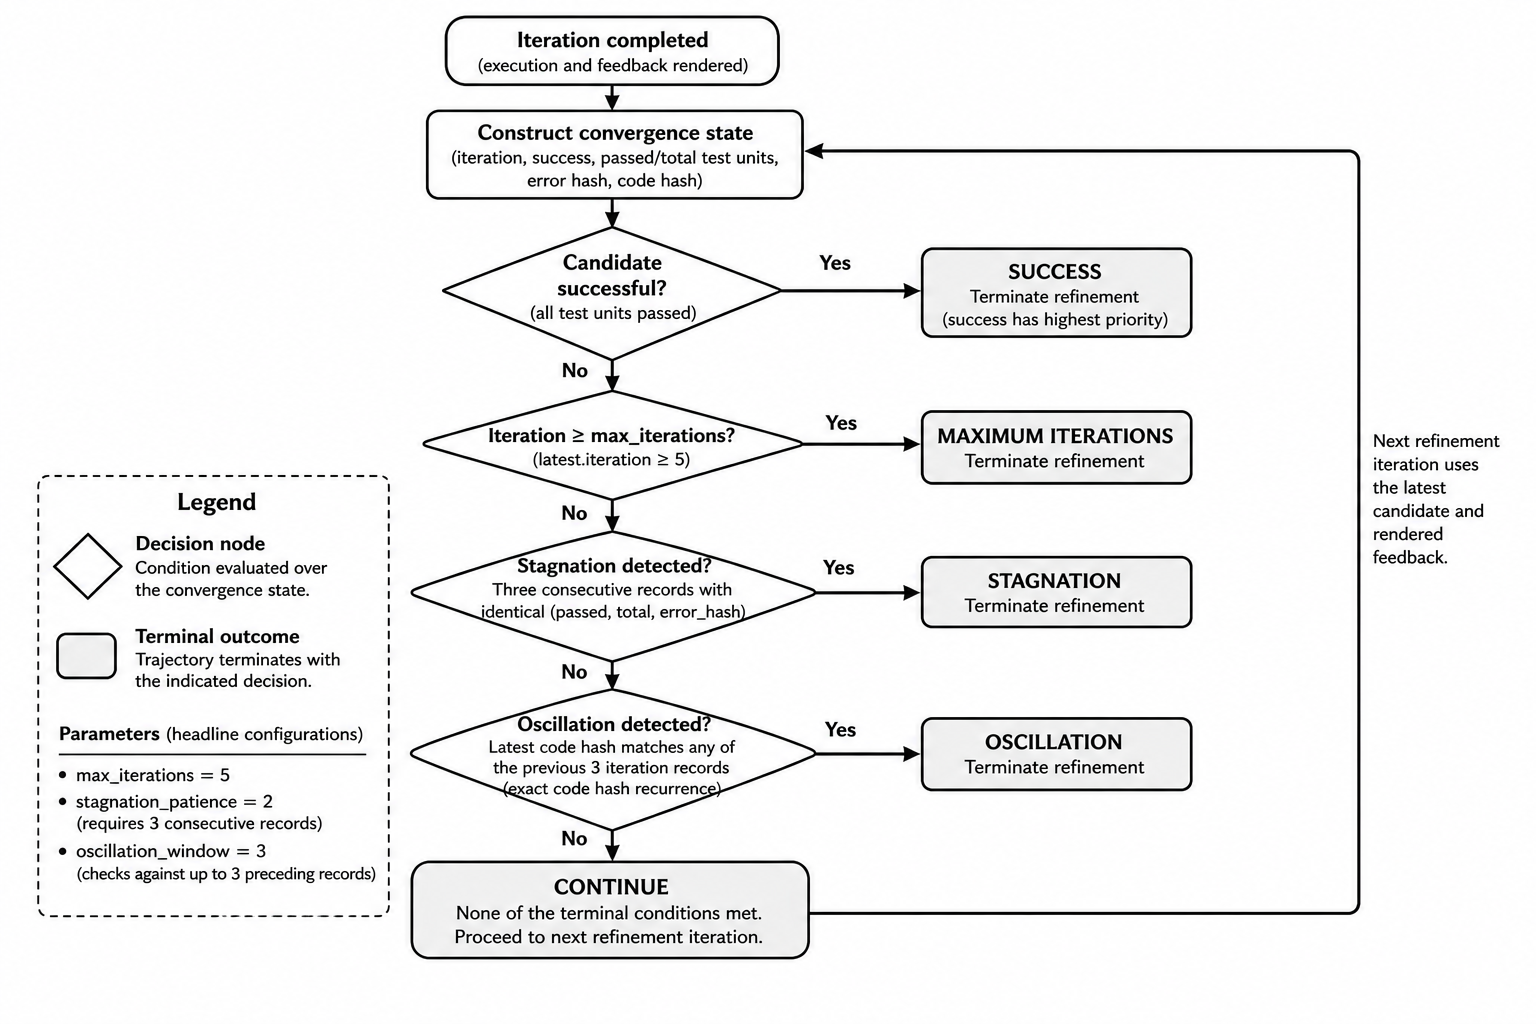
\includegraphics[width=\textwidth]{figures/figure_3_2_adaptive_convergence.png}
    \caption{Adaptive convergence detection and stopping precedence. After each refinement iteration, the accumulated trajectory state is evaluated in the order success, maximum iterations, stagnation and oscillation; refinement continues only when no terminal criterion is satisfied.}
    \label{fig:adaptive-convergence}
\end{figure}

Figure~\ref{fig:adaptive-convergence} summarises this stopping sequence and the headline convergence parameters.

Success is represented in convergence state by a Boolean derived from the execution classification. It is true when the candidate has passed the available benchmark test units and has consequently been classified as successful. Because success has highest priority, adaptive refinement terminates immediately after recording that iteration and requests no further correction generation. This criterion treats benchmark-defined functional correctness as the stopping target; it does not imply correctness beyond the behaviours covered by the tests.

The next check compares the latest one-based iteration number with the configured maximum using a greater-than-or-equal condition. Headline adaptive configurations set this maximum to five. The criterion supplies a hard upper bound even when successive candidates continue to change and neither repetition heuristic fires. Given the stated precedence, an unsuccessful fifth iteration is recorded as maximum iterations even if the same state would also satisfy stagnation or oscillation. The greater-than-or-equal comparison also makes the detector defensive to an externally supplied record whose iteration number has already exceeded the configured bound, although the refinement runner itself generates no more than the configured number of cycles.

Stagnation examines consecutive observable failure states rather than candidate text. For configured patience $p$, the detector requires $p+1$ records and compares the most recent $p+1$ state tuples,
\[
    (n_{\mathrm{pass}},\ n_{\mathrm{total}},\ h_{\mathrm{error}}).
\]
The headline setting is $p=2$, so three consecutive iteration records must contain identical passed counts, total counts and error hashes. The counts are executor test-unit counts and do not necessarily enumerate every assertion inside a compound benchmark harness. The error hash is a SHA-256 digest of the JSON serialisation of the ordered failed-test list. Each list entry contains the exception type, exception message and timeout flag; dictionary keys are serialised in sorted order. Candidate code need not be identical. Stagnation thus denotes recurrence of the same measured test outcome and failure evidence across three records, not merely an unchanged pass rate and not semantic proof that the underlying program has ceased to progress.

Oscillation instead operates on exact extracted source. The runner computes each code hash as the SHA-256 digest of the generated candidate string. After the higher-priority checks, the latest hash is compared with each of up to the preceding three records, reflecting the headline oscillation window of three. Equality with any hash in that recent window terminates the adaptive trajectory as oscillation. The rule therefore detects immediate repetition as well as longer recurrence; it does not require a strict $A\rightarrow B\rightarrow A$ alternation. It also performs neither abstract-syntax-tree comparison nor behavioural equivalence testing: formatting or other source changes produce a different hash, while only exact source repetition qualifies.

When none of the four terminal conditions applies, the detector returns continue. The refinement runner then uses the latest candidate and its deterministic feedback to construct the next dependent revision described in the preceding section. Fixed-$k=5$ refinement deliberately does not call this detector: it follows the same revision pathway but continues until its fifth-iteration completion decision. Adaptive stopping is therefore the manipulated control policy in the convergence ablation, while feedback-conditioned generation is shared between modes.

These criteria are operational heuristics for controlled empirical evaluation rather than theoretically optimal convergence tests. Success avoids unnecessary revision once the benchmark target is met, the maximum bounds inference cost, stagnation identifies repeated observable failure evidence, and oscillation identifies recent exact-code recurrence. Their limitations follow directly from those representations. Stagnation cannot observe semantic intent, and unchanged evidence may reflect incomplete tests rather than a truly exhausted repair path. Oscillation can miss semantically equivalent rewrites, while a continually changing failure state does not establish genuine progress. Benchmark tests may omit behavioural defects, and five iterations is an experimental design choice rather than a universally optimal stopping point.

\section{Experimental Baselines}

The evaluation uses four inference strategies to distinguish the effect of execution-guided repair from the more general benefit of making additional model calls. Single-pass establishes performance under one generation opportunity. Best-of-5 allocates additional opportunities to independent exploration, whereas adaptive refinement allocates up to the same maximum to dependent repair of an evolving candidate. Fixed-$k=5$ refinement retains that repair pathway but removes adaptive stopping. These controls address three separate questions: whether repair improves on one attempt, whether repair is a better allocation of a bounded generation budget than independent sampling, and whether adaptive stopping contributes beyond iterative feedback itself. Table~\ref{tab:experimental-strategies} summarises the controlled distinctions.

Single-pass produces one zero-shot candidate for each task using the experiment's deterministic seed, then executes that candidate once against the benchmark test units. The runner records the generation and execution outcome and completes the task without invoking failure classification, feedback generation or convergence detection. Task success is simply whether this sole candidate passes the available tests. It therefore provides the minimum-compute reference needed to determine what changes when further inference opportunities are introduced, without prejudging whether those opportunities should be used for exploration or repair.

Best-of-5 produces five independent zero-shot candidates per task. Candidate $i$ uses the deterministic seed $s+i$, where $s$ is the experiment base seed and $i\in\{0,\ldots,4\}$. No candidate receives another candidate's code, execution result or feedback. Every candidate is evaluated through the resource-limited subprocess executor, and all five are evaluated even if an earlier sample passes. The task is solved when any candidate passes; there is no voting or selection by frequency. Exact candidate hashes, the number of unique candidates and whether all candidates are unique are retained as sampling-diversity diagnostics. This baseline represents additional inference allocated to independent candidate diversity.

Best-of-5 is generation-budget-matched to the maximum opportunity available to refinement. Best-of-5 and fixed-$k=5$ each make exactly five generation calls per task, while adaptive refinement can make at most five and may stop earlier. The comparison therefore controls for an alternative use of the five-generation allowance, but it is not matched to adaptive refinement's realised call count. Nor does the term imply equal prompt or completion tokens, latency or wall-clock time: refinement prompts contain prior code and feedback, and adaptive stopping deliberately reduces realised computation on some trajectories.

Adaptive refinement begins with the same form of zero-shot attempt used by Single-pass. Following execution, deterministic hybrid feedback conditions a dependent revision on the immediately preceding candidate and observed failure evidence. This pathway repeats for at most five iterations and is terminated by the adaptive convergence policy described in Section~\ref{sec:adaptive-convergence}; success stops the trajectory immediately. Task-level success records whether the trajectory discovers a passing candidate. Because adaptive refinement terminates at its first success, ever-solved and terminal correctness coincide under this protocol.

Fixed-$k=5$ refinement uses the same initial prompt, dependent revision pathway, execution mechanism, deterministic hybrid feedback and five-iteration upper setting as adaptive refinement. It deliberately bypasses the adaptive convergence detector, performs exactly five iterations and continues after an earlier success. Its primary success accounting is therefore ever-solved: whether any iteration discovers a passing candidate. The fifth iteration's correctness remains separately recoverable for final-state and regression diagnostics. Fixed-$k=5$ is a convergence ablation rather than a proposed deployment policy; comparison with adaptive refinement isolates the stopping rule while holding feedback-conditioned revision constant.

\begin{table}[htbp]
    \centering
    \caption{Comparison of the four principal inference strategies.}
    \label{tab:experimental-strategies}
    \small
    \renewcommand{\arraystretch}{1.15}
    \begin{tabular}{p{0.18\textwidth} p{0.30\textwidth} p{0.21\textwidth} p{0.16\textwidth}}
        \hline
        \raggedright Strategy & \raggedright Candidate and feedback structure & \raggedright Stopping policy & \raggedright Maximum generations/task \tabularnewline
        \hline
        \raggedright Single-pass & \raggedright Single candidate; no feedback & \raggedright After first attempt & \raggedright 1 \tabularnewline
        \raggedright Best-of-5 & \raggedright Five independent candidates; no feedback & \raggedright After all five & \raggedright 5 \tabularnewline
        \raggedright Adaptive refinement & \raggedright Dependent revisions; hybrid feedback & \raggedright Adaptive convergence & \raggedright $\leq 5$ \tabularnewline
        \raggedright Fixed-$k=5$ refinement & \raggedright Dependent revisions; hybrid feedback & \raggedright Forced iteration 5 & \raggedright 5 \tabularnewline
        \hline
    \end{tabular}
\end{table}

Within a model--benchmark condition, the strategies share the normalised task representation, model artifact and backend, prompt framework, code extraction, subprocess execution mechanism, test harness and experiment base seed. The five-generation maximum opportunity is common to Best-of-5, adaptive refinement and fixed-$k=5$. Their intentional differences are candidate independence, feedback availability, seed schedule and stopping policy. Best-of-5 also uses the diversity-oriented temperature of 0.8, whereas Single-pass and refinement use 0.2; thus the decoding policy is part of the sampling-versus-repair treatment rather than a fully held-constant variable. The Best-of-5 comparison consequently evaluates a complete independent-sampling policy against a complete feedback-conditioned repair policy; it does not isolate the causal effect of feedback under identical decoding parameters. Prompt lengths likewise diverge once refinement incorporates prior code and feedback. These controls support an exploration-versus-exploitation comparison without claiming exact equality of tokens, latency or realised compute.

A comparison only against Single-pass would be insufficient to attribute a change to execution feedback, because additional calls alone create more opportunities to find a correct program. Best-of-5 supplies the necessary alternative allocation: exploration through independent candidates rather than exploitation through revision of one trajectory. Fixed-$k=5$ then distinguishes the effect of adaptive stopping from the effect of repeated feedback-conditioned generation. Together, the four strategies expose the source of any later difference without assuming in advance that either diversity, repair or early stopping is superior.

\section{Models and Inference Configuration}
\label{sec:models-inference}

The empirical design uses Qwen2.5-Coder-7B-Instruct as the primary model and CodeLlama-13B-Instruct as a cross-model replication. Qwen is evaluated across the complete headline campaign, while CodeLlama repeats the principal conditions to test whether observed behaviours recur under a materially different model configuration. Both are accessed through the common generation interface described in Section~3.3, so task representation, prompt rendering, code extraction and downstream evaluation remain shared. This design broadens the evidence beyond one model, but it does not constitute a controlled model-family ablation: family, parameter scale and numerical representation change together.

Headline Qwen experiments use Hugging Face Transformers with the following frozen model identity:
\begin{center}
    \small\texttt{Qwen/Qwen2.5-Coder-7B-Instruct}\\
    \texttt{revision: c03e6d358207e414f1eca0bb1891e29f1db0e242}
\end{center}
\nopagebreak[4]
The model and tokenizer are loaded on CUDA. The backend uses the bfloat16 dtype, recorded as \texttt{torch.bfloat16} in the persisted evidence. No Hugging Face quantisation option or bitsandbytes configuration is present for these runs. This path is therefore described as non-quantised bfloat16 inference, not IEEE FP32 inference. The distinction is retained when interpreting both memory use and cross-model differences.

Local Qwen development instead uses Ollama with the frozen local artifact:
\begin{center}
    \small\texttt{qwen2.5-coder:7b-instruct-q4\_K\_M}\\
    \scriptsize\texttt{digest: dae161e27b0e90dd1856c8bb3209201fd6736d8eb66298e75ed87571486f4364}
\end{center}
The configuration records Q4\_K\_M quantisation. Before a run, each experiment entry point asks the Ollama backend to verify that the configured model tag is installed, that its reported digest equals the configured digest and that its reported quantisation level is Q4\_K\_M; a mismatch aborts rather than silently substituting another artifact. Requests are sent to the configured local endpoint and retain the same prompt and decoding fields as the cluster path. These runs supported development and validation on local hardware. They are not the headline Qwen evaluation configuration and are not combined with the non-quantised cluster results as though their numerical representations were interchangeable.

The replication model uses Hugging Face Transformers with the following frozen model identity:
\begin{center}
    \small\texttt{codellama/CodeLlama-13b-Instruct-hf}\\
    \texttt{revision: 745795438019e47e4dad1347a0093e11deee4c68}
\end{center}
It is loaded on CUDA with bitsandbytes 8-bit quantisation. The backend translates this setting into \texttt{load\_in\_8bit=true}. Persisted generation provenance identifies the result as quantised and records \texttt{torch.bfloat16} as the backend dtype. This dtype is selected by the shared CUDA backend, while the model parameters are subject to bitsandbytes 8-bit loading. No stronger claim about an exact GPU model, CUDA release, PyTorch release or Transformers release is made because those versions are not recorded consistently in the authoritative run artifacts.

The Qwen--CodeLlama comparison is therefore a replication across models and configurations. Qwen has approximately seven billion parameters and uses non-quantised bfloat16 loading, whereas CodeLlama has approximately thirteen billion parameters and uses bitsandbytes 8-bit quantisation. An absolute difference between their measurements could reflect architecture or training, parameter scale, quantisation, or an interaction among these factors. Recurrence of a refinement behaviour across both configurations supplies evidence that it is not confined to the primary Qwen setting, but the design cannot attribute between-model differences solely to model family or precision.

Where genuinely common, generation is configuration controlled. The headline configurations use the zero-shot prompt strategy, nucleus parameter \(\mathit{top\_p}=0.95\), a maximum of 512 newly generated tokens and repetition penalty 1.1. Hugging Face generation applies the model's chat template, sets sampling whenever temperature is greater than zero, and records the rendered messages, effective generation options and token counts. Thus the headline temperatures of 0.2 and 0.8 use stochastic sampling. The temperature-zero sensitivity condition disables sampling in the Hugging Face backend. Table~\ref{tab:model-inference-config} separates the strategy-specific settings that would be obscured by describing a single common decoding configuration.

Single-pass, adaptive refinement and fixed-$k=5$ refinement use temperature 0.2 for both models. Best-of-5 instead uses temperature 0.8 while retaining \(\mathit{top\_p}=0.95\), the 512-token limit and repetition penalty 1.1. This is an intentional diversity-oriented decoding treatment: Best-of-5 is an independent-sampling comparator, not five decoding-identical repetitions of the lower-temperature policy. Its five candidates use deterministic seeds \(s+i\), where the experiment base seed is \(s=42\) and sample indices are \(i\in\{0,\ldots,4\}\), giving seeds 42--46. This schedule promotes reproducible variation while ensuring that no later candidate depends on an earlier output.

Refinement uses the fixed experiment seed 42 for every generation within a task trajectory. Seed reuse should not be interpreted as requesting identical generations: after the initial zero-shot call, the user prompt changes because it includes the immediately preceding candidate and deterministic execution feedback. The random seed is therefore held constant while the conditioning context evolves. This choice limits an additional source of variation within a dependent repair trajectory, whereas Best-of-5 deliberately varies the seed and withholds preceding candidates and feedback. The distinction is part of the inference treatment and complements the control-flow comparison in Section~3.8.

Temperature sensitivity is evaluated for adaptive hybrid refinement at exactly 0.0, 0.4 and 0.8 for both Qwen and CodeLlama, using the 100-task HumanEval ablation split. Other recorded decoding fields remain at \(\mathit{top\_p}=0.95\), 512 new tokens and repetition penalty 1.1. The conditions test whether refinement behaviour depends on deterministic decoding at temperature zero or on progressively greater sampling variation; they do not alter the model artifact or numerical representation within each model. Separate feedback-length configurations impose ceilings of 100, 200 and 300 words while retaining temperature 0.2. Those ceilings alter the corrective prompt content rather than the backend's sampling mechanism and are therefore detailed with the feedback ablation rather than treated as distinct model configurations.

\begin{table}[htbp]
    \centering
    \caption{Model and inference configurations used in the empirical evaluation.}
    \label{tab:model-inference-config}
    \small
    \renewcommand{\arraystretch}{1.15}
    \begin{tabular}{p{0.24\textwidth} p{0.15\textwidth} p{0.23\textwidth} p{0.08\textwidth} p{0.14\textwidth}}
        \hline
        \raggedright Configuration & \raggedright Backend & \raggedright Numerical representation & \raggedright Temp. & \raggedright Generation note \tabularnewline
        \hline
        \raggedright Qwen Single-pass & \raggedright HF/CUDA & \raggedright Non-quantised bfloat16 & \raggedright 0.2 & \raggedright One call \tabularnewline
        \raggedright Qwen Best-of-5 & \raggedright HF/CUDA & \raggedright Non-quantised bfloat16 & \raggedright 0.8 & \raggedright Five seeds \tabularnewline
        \raggedright Qwen adaptive/fixed refinement & \raggedright HF/CUDA & \raggedright Non-quantised bfloat16 & \raggedright 0.2 & \raggedright Up to/exactly five \tabularnewline
        \raggedright CodeLlama Single-pass & \raggedright HF/CUDA & \raggedright bitsandbytes 8-bit & \raggedright 0.2 & \raggedright One call \tabularnewline
        \raggedright CodeLlama Best-of-5 & \raggedright HF/CUDA & \raggedright bitsandbytes 8-bit & \raggedright 0.8 & \raggedright Five seeds \tabularnewline
        \raggedright CodeLlama adaptive/fixed refinement & \raggedright HF/CUDA & \raggedright bitsandbytes 8-bit & \raggedright 0.2 & \raggedright Up to/exactly five \tabularnewline
        \hline
    \end{tabular}
\end{table}

All headline and Pro configurations preserve these model-specific representations and strategy-specific decoding settings, with configuration snapshots and per-generation request metadata retained in the run evidence. Revisions, seeds, prompts, effective options, accelerator and backend provenance can therefore be audited after execution. Authoritative cluster runs used the University of Surrey AI-NLP01 system with $2\times$ NVIDIA RTX A5000 24GB GPUs. Reproducibility is nevertheless bounded by what was captured: the hardware identity, artifact revisions and inference controls are known, but the complete software-version stack was not uniformly recorded. The model comparison is accordingly strongest as a replication of experimental patterns under two frozen configurations, not as an estimate of a single isolated model-family effect.

\section{Benchmarks and Dataset Validation}
\label{sec:benchmark-validation}

The empirical evaluation uses four Python function-level benchmarks, all converted into the same internal problem representation before generation or execution. HumanEval and sanitised MBPP form the standard headline evaluation, while HumanEval Pro and MBPP Pro provide the harder Tier~3 conditions. The Pro datasets test whether experimental patterns persist as task difficulty increases, but they do not extend the study beyond function-level programming. Table~\ref{tab:benchmark-summary} records the validated matrix. No training or fine-tuning split is constructed from these benchmarks: the headline protocols evaluate all 164 HumanEval tasks and all 427 sanitised MBPP tasks, and the Pro protocols evaluate their complete prepared sets.

HumanEval is acquired from the configured upstream compressed JSON Lines source and retained as 164 uniquely identified tasks. Each source record supplies a task identifier, a prompt containing the Python function declaration and specification, a canonical completion, a test harness and the named entry point. Normalisation concatenates the prompt and completion to form an executable canonical solution and maps the source harness into the common schema. The frozen full-set artifact used by the headline configurations is \texttt{data/normalized/humaneval.jsonl}. It preserves the historical compound harness used for the authoritative full runs, including the call to the recorded entry point. The separately prepared 20-task development subset uses strict AST-based extraction of safe atomic assertions; its validation report records 20 of 20 harnesses split successfully into 148 executable test units. This distinction prevents the later atomic development representation from being retrospectively substituted into the frozen headline evidence.

The second standard benchmark is consistently termed \emph{sanitised MBPP} because acquisition uses the official \texttt{sanitized-mbpp.json} artifact rather than the complete unsanitised collection. Its 427 records contain a natural-language task prompt, reference code, imports, standard assertions and, where present, challenge assertions. Normalisation prefixes required imports to each assertion so that test units remain independently executable. Because this source does not provide a dedicated entry-point field and its prose often omits the required function name, the loader parses both the canonical solution and assertions with the Python AST. It requires exactly one tested top-level function and appends that function's exact signature to the model prompt. The resulting task ID, augmented prompt, canonical solution and test units are written to \texttt{data/normalized/mbpp\_sanitized.jsonl} with the tags \texttt{mbpp} and \texttt{sanitized}. The final artifact contains 427 unique tasks and has a frozen SHA-256 checksum retained in the project audit evidence.

This signature rule arose from a material data-integrity failure. An initial MBPP normalisation copied only the underspecified natural-language prompt and omitted the executable entry-point contract. Generated programs could therefore implement the requested behaviour under a plausible but untested name, producing artificial \texttt{NameError} outcomes when the harness called the expected function. The affected development artifact and runs were invalidated. AST-based signature extraction was then introduced, normalisation was made to fail unless exactly one tested top-level function could be identified, and the development artifact was regenerated without resampling. This incident demonstrates that benchmark normalisation is part of the measurement apparatus: losing the required interface can invalidate model measurements even when the raw reference code and tests are correct.

A later full-set configuration exposed a second provenance failure by referencing a stale, pre-correction normalised MBPP file. The repeated missing-signature pattern was detected before the run was accepted, and that run was excluded. Guard commit \texttt{77f91a7} strengthened \texttt{load\_jsonl()} so that loading a normalised record recomputes the tested signature from its canonical solution and tests, then requires the prompt to contain exactly one matching signature block. The authoritative full artifact was regenerated from the raw sanitised source, and regression tests cover both rejection of the stale form and acceptance of the corrected form. Thus corrected implementation code alone was insufficient: the artifact and its provenance also had to be validated before evaluation.

HumanEval Pro and MBPP Pro are integrated from the MIT-licensed CodeEval-Pro project at pinned revision 36f292eafc597b38535fbc8b4aafea8e5c654e3c. The prepared datasets contain 164 and 378 tasks respectively. Each source record combines a base problem with a dependent problem whose solution must call the first solution. The loader constructs one prompt requesting both complete implementations, combines the two specifications and reference implementations into the canonical program, and splits top-level test assertions into executable units while retaining shared setup code. Records receive benchmark-specific identifiers and tags before entering the same downstream schema. The project treats these as harder benchmark variants; it does not infer undocumented claims about their construction or contamination.

Canonical-solution validation precedes normalized artifact creation for all four datasets. The validator first parses each canonical program with \texttt{ast.parse}, then executes it against its prepared test units through the shared subprocess executor. Failures are logged with their stage and execution evidence to a quarantine file rather than silently repaired or omitted. The build aborts if any quarantine is non-empty or if a source count differs from the required matrix. This procedure established successful validation for 164 of 164 HumanEval Pro records and 378 of 378 MBPP Pro records, alongside the complete standard sets, before authoritative model evaluation. It establishes that the prepared records execute coherently under this harness and that their reference solutions satisfy the available tests; it does not establish benchmark completeness, absence of contamination or correctness beyond those tests.

\begin{table}[htbp]
    \centering
    \caption{Benchmarks and validated task counts used in the empirical evaluation.}
    \label{tab:benchmark-summary}
    \small
    \renewcommand{\arraystretch}{1.15}
    \setlength{\tabcolsep}{4pt}
    \begin{tabular}{p{0.21\textwidth} p{0.08\textwidth} p{0.20\textwidth} p{0.40\textwidth}}
        \hline
        Benchmark & Tasks & Role & Evaluation scope \\
        \hline
        HumanEval & 164 & Standard & Full-set headline evaluation \\
        Sanitised MBPP & 427 & Standard & Full-set headline evaluation \\
        HumanEval Pro & 164 & Harder evaluation & Tier~3 full-set evaluation \\
        MBPP Pro & 378 & Harder evaluation & Tier~3 full-set evaluation \\
        \hline
    \end{tabular}
\end{table}

The common \texttt{Problem} schema stores an exact task ID, model-facing specification, canonical solution, executable test-unit sequence, difficulty value and tags. Normalising to this boundary reduces benchmark-specific variation in later prompt construction, code generation, execution and success accounting. It does not make acquisition identical: HumanEval preserves its entry-point harness, sanitised MBPP reconstructs the tested signature and imports, and CodeEval-Pro combines dependent problem pairs. Dataset-specific transformations are therefore validated before the shared pipeline begins rather than being hidden by the common representation.

Development and sensitivity data are kept distinct from full-set evaluation. HumanEval-Dev contains 20 tasks and MBPP-Dev 50 tasks, selected reproducibly with seed 42. Because the standard records expose only one difficulty/tag stratum, the splitter proportionally samples task-ID rank quartiles rather than inventing difficulty labels.

The sensitivity artifact is \texttt{data/dev/humaneval\_ablation\_100.jsonl}. It is a fixed 100-task stratified HumanEval subset constructed with the same seed and reused across feedback-length and temperature conditions, so sample composition cannot explain differences among those configurations.

These safeguards do not remove the benchmarks' scope limitations. Every evaluated task is a Python function-level problem, and passing the available tests operationalises functional correctness only for covered behaviours. Test coverage and granularity vary, so a passing candidate is not proof of broader semantic correctness. Findings do not automatically generalise to repository-level maintenance, multi-file systems or production software engineering. Moreover, the MBPP incidents show that validity depends on acquisition, normalisation and harness construction as well as on the benchmark source itself; explicit counts, canonical execution, invariants, quarantine and provenance checks are therefore necessary parts of the evaluation methodology.

\section{Experimental Campaign}
\label{sec:experimental-campaign}

The authoritative experimental campaign is organised as a matrix rather than a chronological sequence of runs. It expands the primary comparison along three principal dimensions: inference strategy, model configuration and benchmark difficulty. Controlled sensitivity conditions then examine whether selected inference-level choices materially alter the adaptive-refinement procedure. Across the core campaign, the four principal strategies defined in Section~3.8---Single-pass, Best-of-5, Adaptive refinement and Fixed-$k=5$ refinement---are applied consistently. Table~\ref{tab:experimental-campaign} summarises this structure without duplicating their control-flow definitions.

Tier~1 establishes the primary standard-benchmark comparison using Qwen2.5-Coder-7B-Instruct. The two benchmark conditions are the complete HumanEval set of 164 tasks and the complete sanitised MBPP set of 427 tasks described in Section~\ref{sec:benchmark-validation}. Crossing two benchmarks with four inference strategies yields eight authoritative configurations. This stage provides the central evidence for assessing whether execution-feedback refinement improves upon a single generation, how it compares with generation-budget-matched sampling, and whether adaptive stopping changes the cost and outcome of refinement. It therefore supplies the primary-model basis for RQ1--RQ3 before any cross-configuration replication is considered.

Tier~2 repeats the same two-benchmark, four-strategy matrix with CodeLlama-13B-Instruct, adding a further eight configurations. Holding the higher-level experimental pipeline and task sets constant makes this a cross-model and cross-configuration replication of the qualitative comparisons examined in Tier~1. It is not a clean model-family ablation: as established in Section~\ref{sec:models-inference}, CodeLlama also differs from Qwen in parameter scale and uses bitsandbytes 8-bit loading rather than non-quantised bfloat16. Conclusions from this stage must consequently concern replication across the two evaluated configurations, not an isolated causal effect of model family.

Tier~3 Pro extends the design along the benchmark-difficulty dimension. Both model configurations are evaluated on HumanEval Pro (164 tasks) and MBPP Pro (378 tasks), again under all four principal strategies. The resulting $2 \times 2 \times 4=16$ configurations test whether behaviour identified on standard HumanEval and sanitised MBPP persists for the harder prepared benchmark variants. This separates sensitivity to benchmark difficulty from conclusions based only on the standard sets and extends the evidence relevant to RQ2 and RQ4. The Pro campaign remains a function-level evaluation and is not treated as evidence for repository-scale generalisation.

The sensitivity campaign comprises twelve additional reporting configurations on the fixed 100-task HumanEval ablation subset. For each model, adaptive hybrid refinement is evaluated under three feedback-length caps (100, 200 and 300 words) and three temperatures (0.0, 0.4 and 0.8). Thus each model contributes six conditions and the two models contribute twelve. Reusing the same task subset and seed across these conditions prevents task-composition changes from confounding their comparison. Section~3.12 specifies the sensitivity design in detail; its role here is to complete the campaign accounting after the model and difficulty extensions.

\begin{table}[htbp]
    \centering
    \caption{Structure of the final authoritative experimental campaign.}
    \label{tab:experimental-campaign}
    \footnotesize
    \renewcommand{\arraystretch}{1.15}
    \setlength{\tabcolsep}{3pt}
    \begin{tabular}{p{0.11\textwidth} p{0.18\textwidth} p{0.20\textwidth} p{0.25\textwidth} p{0.12\textwidth}}
        \hline
        \raggedright Campaign stage & \raggedright Model configuration(s) & \raggedright Benchmark(s) & \raggedright Conditions & \raggedright \scriptsize Configurations \tabularnewline
        \hline
        \raggedright Tier 1 & \raggedright Qwen & \raggedright HumanEval; sanitised MBPP & \raggedright Four principal strategies & \raggedright 8 \tabularnewline
        \raggedright Tier 2 & \raggedright CodeLlama & \raggedright HumanEval; sanitised MBPP & \raggedright Four principal strategies & \raggedright 8 \tabularnewline
        \raggedright Tier 3 Pro & \raggedright Qwen and CodeLlama & \raggedright HumanEval Pro; MBPP Pro & \raggedright Four principal strategies & \raggedright 16 \tabularnewline
        \raggedright Sensitivity & \raggedright Qwen and CodeLlama & \raggedright HumanEval 100-task subset & \raggedright Three feedback lengths and three temperatures per model & \raggedright 12 \tabularnewline
        \hline
        \multicolumn{4}{l}{Total authoritative reporting configurations} & \raggedright 44 \tabularnewline
        \hline
    \end{tabular}
\end{table}

The final reporting total follows directly from the matrix:
\[
8 + 8 + 16 + 12 = 44.
\]
These 44 configurations, comprising 32 core and 12 sensitivity configurations, are the complete authoritative set used for dissertation reporting. The arithmetic also provides a reproducible boundary around the evidential scope: configurations retained for development, validation or audit purposes cannot enter headline comparisons merely because their artifacts remain available.

This boundary is necessary because the repository contains 86 committed result directories, not 86 reporting experiments. The frozen inventory partitions them into 44 authoritative reporting configurations, 25 development or validation runs, and 17 invalid, incomplete, duplicated or superseded artifacts, satisfying $44+25+17=86$. The 25 supporting runs cover activities such as development-subset evaluation, smoke tests, local quantised validation, interface checks, corrected validation runs and methodological verification. They establish that components and execution environments behaved as intended, but they are not substituted for frozen reporting configurations. Likewise, excluded artifacts remain available as an audit trail rather than being deleted or silently reclassified. Only the 44 authoritative configurations contribute to final experimental reporting; the dataset-specific integrity incidents motivating some exclusions are addressed in Section~\ref{sec:benchmark-validation}, while the wider evidence audit is reserved for the reproducibility and integrity discussion.

Authoritative configurations were frozen before final reporting and executed as predefined YAML specifications rather than through manual parameter changes during a run. Each run directory preserves its resolved configuration, deterministic seeds and Git commit provenance alongside per-problem records and aggregate summaries. Model revisions and backend settings are therefore attributable to the configuration that produced each record. Completed-problem records are written incrementally and atomically, and resume validation requires the stored configuration to match before complete records can be reused. These controls support long-running execution without implying that interrupted problems resume midway through a trajectory.

The cluster exposed two GPUs, which were used in parallel for portions of Tier~3 by assigning independent configurations explicitly to individual devices. This was an operational scheduling decision: configurations did not combine GPUs or share model state, and their recorded model, dataset, seed and execution protocols were unchanged. Access to GPU~1 remained conditional on a three-sample sustained-idleness preflight. With supervisory approval, its utilisation threshold was raised from 5\% to 25\% to accommodate display activity, while the 500~MiB memory threshold and refusal-on-failure safeguards remained active. Parallel scheduling therefore affected campaign throughput, not the statistical definition of any task outcome.

\section{Sensitivity and Ablation Design}
\label{sec:sensitivity-design}

The sensitivity campaign evaluates the robustness of adaptive execution-feedback refinement to two distinct inference-level design choices. Feedback-length sensitivity varies the information budget available for corrective diagnostics in the next prompt, whereas temperature sensitivity varies the stochastic sampling behaviour of the generation backend. These manipulations are robustness analyses, not a generic hyperparameter search or optimisation for deployment, and they were not used retrospectively to select or redefine the headline configuration. Instead, they test whether the observed refinement behaviour depends materially on how much rendered execution evidence is supplied and on how candidates are sampled, thereby addressing the inference-settings component of RQ4.

The design changes one focal variable within each family while preserving its remaining controls. Comparisons are consequently intended primarily within the three feedback ceilings or within the three temperature settings. The two families are complementary rather than directly interchangeable treatments because the temperature configurations do not impose the explicit word ceiling used by the feedback-length configurations.

Every condition uses the fixed HumanEval ablation artifact at \path{data/dev/humaneval_ablation_100.jsonl}. The subset contains 100 tasks selected reproducibly with seed 42 through the project's stratified splitter; because the normalised HumanEval records form one semantic stratum, selection is proportionally distributed across task-ID rank quartiles. The same task IDs are used in all twelve configurations and for both model configurations. Holding task composition fixed prevents sample-selection differences from being mistaken for sensitivity to feedback length or temperature. This subset supports controlled analysis and is not an additional headline benchmark.

\subsection{Feedback-Length Sensitivity}

Feedback length is controlled after the configured hybrid strategy has classified the execution outcome and rendered its template- or trace-oriented diagnostic. The factory wraps the hybrid generator in a deterministic \texttt{BoundedFeedbackGenerator}. This wrapper splits the rendered string on whitespace and retains at most the configured number of words before joining them for the next refinement prompt. The operation is therefore word-based truncation, not token-level clipping, semantic summarisation, adaptive compression or LLM-based shortening. Its delegated \texttt{strategy\_for} method preserves the effective template or trace label in the per-iteration evidence even when the associated feedback text is bounded.

The three ceilings are 100, 200 and 300 words. They represent, respectively, a more constrained corrective signal, an intermediate information budget and a less restrictive ceiling; 300 words is not assumed to be unrestricted, and no ordering of expected effectiveness is imposed. The manipulation changes only the amount of rendered diagnostic content admitted to the next prompt. Failure classification, hybrid routing, underlying execution evidence and adaptive convergence logic remain unchanged.

Within this family, both models use temperature 0.2, \(\mathit{top\_p}=0.95\), a maximum of 512 new tokens, repetition penalty 1.1 and seed 42. All configurations use hybrid feedback, adaptive convergence, a maximum of five iterations, stagnation patience two and oscillation window three. They also share the prompt framework, subprocess executor, test harness and fixed benchmark subset. The model artifact remains fixed within each model: the Qwen and CodeLlama conditions use their respective pinned revisions and the numerical representations defined in Section~\ref{sec:models-inference}.

\subsection{Temperature Sensitivity}

Temperature sensitivity evaluates the same adaptive hybrid-refinement procedure at 0.0, 0.4 and 0.8. In the Hugging Face generation path, \texttt{do\_sample} is set from whether temperature is greater than zero. Temperature 0.0 consequently disables stochastic sampling, while 0.4 and 0.8 enable sampling with progressively higher configured temperature. This design tests increasing sampling variation relative to the zero-temperature path without claiming measured monotonic diversity or guaranteeing identical generations at temperature 0.0.

The temperature configurations retain \(\mathit{top\_p}=0.95\), the 512-token generation limit, repetition penalty 1.1 and seed 42. They also hold constant the model revision within each model, fixed task subset, prompt construction, executor and tests, hybrid routing, adaptive convergence settings and five-iteration allowance. Unlike the feedback-length family, these configurations do not set \texttt{feedback\_max\_words}; its resolved value is null, so the factory uses the hybrid generator without the bounded-word wrapper. This distinction prevents the methodology from falsely asserting one common feedback ceiling across both sensitivity families.

\begin{table}[htbp]
    \centering
    \caption{Sensitivity conditions used for adaptive hybrid refinement.}
    \label{tab:sensitivity-design}
    \footnotesize
    \renewcommand{\arraystretch}{1.15}
    \setlength{\tabcolsep}{3pt}
    \begin{tabular}{p{0.17\textwidth} p{0.20\textwidth} p{0.29\textwidth} p{0.18\textwidth}}
        \hline
        \raggedright Sensitivity family & \raggedright Conditions & \raggedright Fixed benchmark subset & \raggedright Models \tabularnewline
        \hline
        \raggedright Feedback length & \raggedright 100, 200 and 300 words & \raggedright HumanEval ablation subset (100 tasks) & \raggedright Qwen and CodeLlama \tabularnewline
        \raggedright Temperature & \raggedright 0.0, 0.4 and 0.8 & \raggedright HumanEval ablation subset (100 tasks) & \raggedright Qwen and CodeLlama \tabularnewline
        \hline
    \end{tabular}
\end{table}

Each family therefore contributes three conditions for each of two models, giving six feedback-length and six temperature configurations: \((3+3)\times2=12\). Applying the same design to Qwen2.5-Coder-7B-Instruct and CodeLlama-13B-Instruct tests whether sensitivity patterns recur across materially different model configurations. It remains a cross-configuration replication rather than a causal model-family ablation because model family, parameter scale and numerical representation differ. Together with the harder-benchmark extension in Section~\ref{sec:experimental-campaign}, these controlled settings delimit the model-, difficulty- and inference-setting dimensions over which RQ4 is evaluated without prejudging the results.

\section{Evaluation Metrics and Statistical Analysis}
\label{sec:evaluation-metrics}

Functional correctness is measured as a binary task-level outcome determined by the benchmark tests. For Single-pass, a task is solved if its sole generated candidate passes every required test. For Best-of-5, it is solved if at least one of the five independently generated candidates passes, irrespective of the outcomes of the other candidates. For adaptive refinement, a task is solved if any candidate in its refinement trajectory passes. Because adaptive refinement terminates immediately upon success, its ever-solved outcome and its terminal success outcome coincide. For fixed-$k=5$ refinement, the primary solution-discovery outcome is instead ever-solved: a task is credited when any of the five iterations passes. Final-iteration correctness is retained as a separate diagnostic because forced continuation can replace an earlier correct candidate with a failing one.

For a configuration evaluated on $n$ tasks, the reported pass@1 is the empirical success proportion
\[
    \widehat{p}=\frac{1}{n}\sum_{i=1}^{n} y_i,
\]
where $y_i=1$ when task $i$ is solved under the strategy-specific definition above and is zero otherwise. It is therefore the number of solved tasks divided by the total number evaluated under the frozen deterministic protocol. This terminology does not denote the unbiased pass@$k$ estimator sometimes used for repeated code samples. In particular, Best-of-5 first reduces its five candidate outcomes to one any-success task outcome; the proportion of those task outcomes is reported as the strategy's pass@1 measure, not as pass@5.

Efficiency is characterised using total model calls, prompt tokens, completion tokens and wall-clock time. Model calls count generation frequency and are especially informative for the generation-budget-matched comparison: Best-of-5 and fixed-$k=5$ use five generation opportunities per task, whereas adaptive refinement can use fewer by terminating early. Prompt and completion tokens measure the model-facing sequence workload accumulated across those calls. Wall-clock time records realised end-to-end duration, including effects of the execution environment and scheduling. These quantities are complementary rather than interchangeable measures of compute; floating-point operations, energy consumption and monetary cost were not measured.

Comparisons between strategies on a common benchmark are paired by exact task ID. For methods $A$ and $B$, the resulting $2\times2$ table comprises tasks solved by both, solved by $A$ only, solved by $B$ only and solved by neither. The two discordant cells---$b$, the number solved only by $A$, and $c$, the number solved only by $B$---identify both the direction and strength of task-level changes. Identical task-ID sets are required before a paired comparison is computed.

The null hypothesis of equal marginal task-success probabilities is tested using the exact conditional two-sided McNemar test. Conditional on $b+c$ discordant tasks, the implementation evaluates a binomial distribution with success probability $0.5$ and doubles the lower-tail probability at $\min(b,c)$, capped at one. When no discordant tasks exist, the $p$-value is one. Only discordant outcomes contribute to this test; concordant outcomes establish the paired table but do not provide evidence of a difference between its margins. The exact form avoids reliance on a large-sample chi-squared approximation when discordant counts are small, and the two-sided alternative does not prespecify which strategy must perform better. No continuity correction is applied.

Effect size is reported alongside the test result. The paired risk difference is the success proportion for $A$ minus that for $B$, preserving the direction of the named comparison. The matched odds ratio is based on the discordant ratio $b/c$. If either discordant cell is zero, the reported finite ratio applies the implemented Haldane--Anscombe adjustment, $(b+0.5)/(c+0.5)$, and the output explicitly flags that adjustment; the unadjusted ratio is retained only when defined. These effect sizes are part of the frozen paired-statistics output, including the Tier~3 analysis, and are interpreted with the underlying discordant counts rather than in isolation.

Uncertainty in each configuration's task-success proportion is estimated by a problem-level non-parametric percentile bootstrap. Each of 10,000 resamples draws $n$ complete binary task outcomes with replacement from the observed $n$-task vector and recomputes the solved proportion. Seed 42 fixes the resampling sequence. The 95\% interval uses the empirical 0.025 and 0.975 quantiles, calculated by linear interpolation at position $(R-1)q$ for the ordered $R=10{,}000$ bootstrap estimates. These intervals represent sampling uncertainty over the evaluated problem set under the fixed inference protocol. They do not incorporate variation from alternative generation seeds, model training, benchmark contamination, hardware, scheduling or model family.

Table~\ref{tab:evaluation-metrics} summarises the measures and their analytical roles. All paired $p$-values are reported without adjustment for multiplicity and use the prespecified significance level $\alpha=0.05$. They are therefore condition-specific evidence, not family-wise-error-controlled claims across the complete campaign. Statistical significance is considered jointly with absolute solved-task and pass-rate differences, the direction of discordant task flips, model calls, token usage where available, wall-clock behaviour and consistency across benchmarks and model configurations. A $p$-value below 0.05 does not by itself establish practical superiority.

\begin{table}[htbp]
    \centering
    \caption{Evaluation measures used in the empirical analysis.}
    \label{tab:evaluation-metrics}
    \footnotesize
    \renewcommand{\arraystretch}{1.12}
    \setlength{\tabcolsep}{3pt}
    \begin{tabular}{p{0.18\textwidth} p{0.42\textwidth} p{0.27\textwidth}}
        \hline
        \raggedright Measure & \raggedright Definition & \raggedright Primary analytical role \tabularnewline
        \hline
        \raggedright Solved/pass@1 & \raggedright Strategy-specific binary success, aggregated as solved tasks divided by evaluated tasks & \raggedright Functional correctness \tabularnewline
        \raggedright Model calls & \raggedright Number of candidate-generation invocations & \raggedright Generation opportunity and stopping cost \tabularnewline
        \raggedright Prompt/completion tokens & \raggedright Tokens submitted to and returned by the model & \raggedright Model-facing sequence workload \tabularnewline
        \raggedright Wall-clock time & \raggedright Realised end-to-end elapsed time & \raggedright Operational efficiency \tabularnewline
        \raggedright Exact McNemar test & \raggedright Two-sided exact inference from discordant paired task outcomes & \raggedright Condition-specific paired evidence \tabularnewline
        \raggedright Bootstrap interval & \raggedright 95\% problem-level percentile interval from 10,000 resamples & \raggedright Uncertainty in the success proportion \tabularnewline[4pt]
        \raggedright Regression count & \raggedright Previously passing fixed-$k$ trajectory whose fifth iteration fails & \raggedright Cost of forced continuation \tabularnewline
        \hline
    \end{tabular}
\end{table}

Convergence analysis further records adaptive and fixed-$k$ model calls, the additional calls incurred by fixed continuation, ever-solved count, final-iteration solved count and regression count. A regression is counted at the problem-run level when a fixed-$k=5$ trajectory passes at least once before iteration five but its fifth iteration fails; it is not a count of every intermediate pass-to-fail transition. Where a regression proportion is reported, its denominator is the fixed-run tasks that passed at least once. The distinction between ever-solved and final-iteration correctness consequently measures solution discovery separately from the stability of a forcibly continued trajectory.

Feedback-length and temperature sensitivity conditions use these same correctness and efficiency definitions on the identical fixed 100-task subset. Inferential comparisons are restricted to aligned task sets and conditions. In particular, no paired test is formed between HumanEval and MBPP, whose task identities differ. Cross-model patterns are treated as replication and robustness evidence across the two evaluated configurations, rather than as automatically paired causal estimates of model-family effects.

\section{Reproducibility and Experimental Integrity}
\label{sec:reproducibility-integrity}

Reproducibility was treated as traceability from each reported aggregate to a frozen configuration and its constituent task trajectories. At run creation, the fully resolved typed configuration is written as a YAML snapshot alongside the generation seeds and Git commit identifier. Each completed task record preserves model and backend provenance together with the generated code, raw response, rendered prompts, token counts, execution outcome, timing and, where applicable, classification, feedback and convergence state. Run-level CSV and JSON summaries are then derived from those records. This structure permits a reported count to be audited against individual candidates and the configuration that generated them, while avoiding the stronger claim that every historical software and hardware dependency was captured completely.

Avoidable experimental variation was constrained through a base seed of 42, frozen task sets, pinned model revisions and deterministic control logic. Best-of-5 uses the reproducible schedule $42+i$ for sample indices $i=0,\ldots,4$, whereas every generation within a refinement trajectory receives the fixed base seed; successive refinement candidates differ through the preceding code and feedback rather than an iteration-specific seed. The 100-task sensitivity subset is likewise fixed, and failure classification, feedback rendering and convergence decisions are deterministic functions of persisted execution evidence. These controls support rerunning a fixed protocol, but do not guarantee bitwise-identical generation across arbitrary accelerator, library or backend versions.

Long-running campaigns are recoverable at completed-problem granularity. A problem record is written only after its strategy reaches a terminal state, using a temporary file followed by an atomic replacement. On resume, the stored configuration must equal the active resolved configuration before any prior record can be considered. Existing JSON is then checked for the expected task ID, metric, seeds and strategy-specific terminal structure. A valid completed record is reused; a missing, corrupt, incomplete or inconsistent record is regenerated from its first generation. Resume therefore reduces the cost of interrupted full-benchmark runs without constituting a checkpoint after each iteration: neither an interrupted candidate sequence nor a partially completed trajectory is restored midway.

Model identity and evaluation-artifact identity are both guarded. The local Ollama backend requires the configured Qwen tag and verifies its immutable digest and declared quantisation level before use. Hugging Face configurations use full 40-character revision hashes, which are passed to both tokenizer and model loading, while per-record provenance records the realised precision and backend metadata. Normalised datasets are frozen separately from acquisition sources, checked for expected record counts and unique task identifiers, parsed for valid canonical code, and validated by executing canonical solutions against their own tests. The MBPP loader additionally recomputes the tested entry-point signature and rejects any normalised prompt that does not contain exactly one matching signature block. Task-ID equality is enforced before paired statistical comparisons. These mechanisms provide targeted identity and validity checks; they do not imply that every project artifact is content-addressed.

Two MBPP incidents demonstrate why derived benchmark data form part of the measurement apparatus. First, the original sanitised-MBPP normalisation retained an underspecified natural-language prompt but omitted the function signature recoverable from the reference solution and tests. Candidates could consequently implement the intended behaviour under an untested name, producing artificial \texttt{NameError} failures. Those development runs were marked invalid and superseded. AST-based extraction was introduced to require exactly one tested top-level function and append its signature to the prompt, with canonical execution and regression tests validating the corrected artifact. Second, a later full-set configuration still referenced a pre-correction normalised file, so the same failure mode recurred despite the source-code fix. That run was excluded, the 427-task artifact was regenerated, and guard commit \texttt{77f91a7} added the load-time signature invariant. The lesson is that corrected implementation code is insufficient when a configuration can still select stale derived data; Section~\ref{sec:benchmark-validation} documents the dataset mechanics in detail.

A separate integrity audit identified a feedback-fidelity defect in the compound harnesses used by the frozen full-set HumanEval representation. When a later assertion failed, the feedback fallback could display the first textual assertion rather than the assertion identified by the traceback. MBPP was unaffected because its assertions were already atomic; a direct audit found all 1,866 stored MBPP assertion citations matched their failed atomic tests. HumanEval compound-harness handling was changed to recover the traceback-matched assertion, and a regression test covers a harness whose failing assertion is not first. The affected full HumanEval adaptive and fixed-$k=5$ refinement conditions were rerun, and the corrected trajectories superseded the confounded records. Although the adaptive aggregate happened to remain unchanged, paired problem outcomes changed, while fixed-$k$ aggregate and final-iteration outcomes also changed. The defect therefore cannot be dismissed from aggregate equality alone; only corrected outputs enter final reporting. Detailed mismatch rates and paired changes remain in the dedicated validation audit rather than being repeated here.

These corrections instantiate a common evidence-governance rule: once a methodological or data defect was confirmed, affected evidence was labelled invalid or superseded, the underlying mechanism was corrected, a guard or regression test was added, and authoritative conditions were regenerated where necessary. Historical artifacts were retained when appropriate to preserve the audit trail, but were not silently mixed with final evidence. The frozen inventory contains 86 committed result directories: 44 authoritative reporting configurations, 25 development or validation runs, and 17 invalid, incomplete, duplicated or superseded artifacts, satisfying $44+25+17=86$. Only the 44 configurations defined in Section~\ref{sec:experimental-campaign} support final empirical claims.

The final closeout at commit \texttt{db4fa23} records 154 automated tests passing. At a high level, the suite covers dataset loading and guards, generation and extraction, execution, feedback, convergence, persistence and resume, GPU safety and statistical analysis. Passing tests support implementation integrity but do not validate the dissertation's empirical conclusions. Operational safeguards also required GPU~1 to remain below the approved 25\% utilisation and 500~MiB memory thresholds for three consecutive samples, failing closed otherwise. The deliberate use of the resource-limited subprocess executor, rather than Docker, is separately preserved in the sandboxing decision record and is not treated as an undocumented shortcut.

OpenAI Codex supported software development through code generation, debugging and mechanical LaTeX assistance. Research problem formulation, architecture, experimental design, benchmark and model selection, refinement methodology, evaluation protocol, interpretation and dissertation argumentation remained the author's responsibility. AI-assisted code was reviewed and subjected to execution-based validation and automated testing before inclusion.

The resulting evidence is strongly traceable rather than perfectly environment-reproducible. The AI-NLP01 hardware identity is known, but complete software versions were not recorded uniformly; third-party backends may evolve, and identical seeds need not produce identical bits across changed numerical environments. Resume is deliberately problem-granular, historical excluded artifacts remain visible, and correctness remains bounded by the frozen benchmark tests. These limitations qualify environmental replication without weakening the provenance boundary that separates corrected authoritative evidence from the wider audit inventory.

\chapter{Results}

\section{Results Overview and Reporting Conventions}

This chapter reports the empirical outcomes from the 44 authoritative configurations defined in Chapter~3: 32 core configurations and 12 sensitivity configurations. The remaining committed run directories---25 development or validation runs and 17 invalid, incomplete, duplicated or superseded runs---do not contribute to the results reported here. Functional correctness is expressed as both the number of tasks solved and the corresponding problem-level pass@1. Here, pass@1 denotes the strategy-level task success proportion under the frozen protocol: Single-pass requires its sole candidate to pass, Best-of-5 requires any of its five candidates to pass, adaptive refinement requires any candidate in its trajectory to pass, and fixed-$k=5$ uses ever-solved as its principal discovery outcome. For fixed-$k=5$ refinement, the principal discovery outcome is whether a task was solved at any iteration; correctness at iteration five is reported separately as a stability diagnostic.

The primary Qwen2.5-Coder-7B-Instruct configuration used non-quantised bfloat16 inference through Hugging Face/CUDA. The replication configuration used CodeLlama-13B-Instruct with bitsandbytes 8-bit loading through Hugging Face/CUDA. Differences between these configurations are therefore reported as cross-configuration observations. They do not isolate model family, parameter scale or numerical representation.

Best-of-5 and refinement were generation-budget-matched in the sense that each permitted at most five generations per task. Their realised computation was not identical: Best-of-5 always generated five independent candidates at temperature 0.8 using seeds 42--46, whereas adaptive refinement used temperature 0.2, seed 42 within each trajectory and could terminate before its fifth generation. Their comparison consequently evaluates two complete inference policies rather than the isolated causal effect of execution feedback under identical decoding settings. Model calls are used as the principal main-text efficiency measure; they count generation requests and are not treated as equivalent to floating-point operations, latency or energy use.

\section{Standard-Benchmark Functional Correctness}

Table~\ref{tab:standard-results} presents the standard-benchmark results, while Figure~\ref{fig:standard-pass} shows the corresponding pass@1 values. Fixed-$k=5$ is omitted from this headline table and figure because its ever-solved outcome was identical to adaptive refinement in every standard condition; that ablation is examined separately in Section~4.6.

\begin{table}[htbp]
    \centering
    \caption{Functional correctness and model calls on the standard benchmarks. Percentages are problem-level pass@1; counts in parentheses are solved tasks.}
    \label{tab:standard-results}
    \scriptsize
    \renewcommand{\arraystretch}{1.15}
    \resizebox{\textwidth}{!}{%
    \begin{tabular}{llrrrrr}
        \hline
        Model configuration & Benchmark & Single-pass & Best-of-5 & Adaptive & Adaptive calls & BO5 calls \\
        \hline
        Qwen bfloat16 & HumanEval & 86.59\% (142/164) & 92.68\% (152/164) & 90.24\% (148/164) & 199 & 820 \\
        Qwen bfloat16 & Sanitised MBPP & 71.90\% (307/427) & 78.92\% (337/427) & 82.44\% (352/427) & 647 & 2,135 \\
        CodeLlama 8-bit & HumanEval & 41.46\% (68/164) & 62.20\% (102/164) & 53.05\% (87/164) & 311 & 820 \\
        CodeLlama 8-bit & Sanitised MBPP & 44.96\% (192/427) & 61.59\% (263/427) & 60.19\% (257/427) & 821 & 2,135 \\
        \hline
    \end{tabular}}
\end{table}

\begin{figure}[htbp]
    \centering
    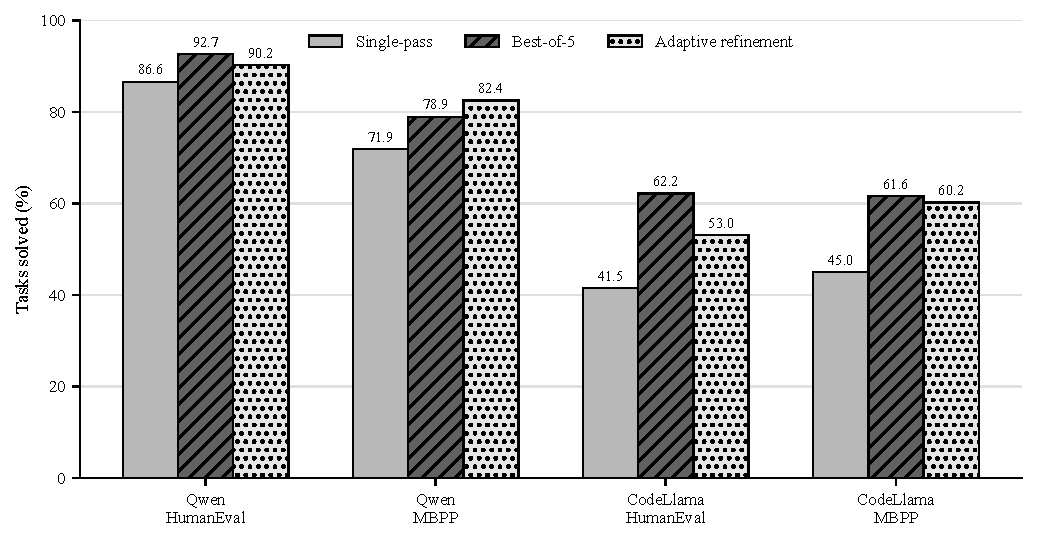
\includegraphics[width=\textwidth]{figures/figure_4_1_standard_pass_at_1.pdf}
    \caption{Problem-level pass@1 for the three principal discovery policies on HumanEval and sanitised MBPP. Qwen denotes non-quantised bfloat16 inference and CodeLlama denotes bitsandbytes 8-bit inference.}
    \label{fig:standard-pass}
\end{figure}

\subsection{Qwen Results}

On HumanEval, Qwen single-pass generation solved 142 of 164 tasks (86.59\%). Best-of-5 increased this to 152 tasks (92.68\%), the highest result in this condition. Adaptive refinement solved 148 tasks (90.24\%): six more than single-pass, but four fewer than Best-of-5. It reached this outcome with 199 model calls, compared with 164 for single-pass and 820 for Best-of-5.

The Qwen ranking changed on sanitised MBPP. Single-pass solved 307 of 427 tasks (71.90\%) and Best-of-5 solved 337 (78.92\%). Adaptive refinement solved 352 tasks (82.44\%), improving on single-pass by 45 tasks and on Best-of-5 by 15. The adaptive procedure used 647 calls, compared with 2,135 for Best-of-5. Thus Qwen adaptive refinement was the highest-scoring of the three policies on sanitised MBPP, whereas Best-of-5 remained highest on HumanEval.

\subsection{CodeLlama Replication}

For CodeLlama on HumanEval, single-pass solved 68 of 164 tasks (41.46\%), Best-of-5 solved 102 (62.20\%), and adaptive refinement solved 87 (53.05\%). Refinement therefore recovered 19 additional tasks relative to single-pass but remained 15 tasks below Best-of-5. Adaptive refinement used 311 calls rather than Best-of-5's 820.

On sanitised MBPP, CodeLlama single-pass solved 192 of 427 tasks (44.96\%). Best-of-5 solved 263 (61.59\%), while adaptive refinement solved 257 (60.19\%). The six-task numerical deficit for adaptive refinement was substantially smaller than its 15-task HumanEval deficit. Adaptive refinement used 821 calls, 1,314 fewer than Best-of-5. This MBPP outcome did not reproduce the Qwen result in which refinement exceeded Best-of-5, but it did reproduce improvement over single-pass and a lower realised call count than five independent samples.

\subsection{Cross-Configuration Pattern}

Across both evaluated configurations and both standard benchmarks, adaptive refinement improved on single-pass: by 3.66 and 10.54 percentage points for Qwen on HumanEval and MBPP, and by 11.59 and 15.22 points for CodeLlama. Its ranking relative to Best-of-5 was not uniform. It trailed Best-of-5 in three conditions and led in Qwen sanitised MBPP. Figure~\ref{fig:standard-pass} also shows that the absolute pass@1 levels differed substantially between model configurations. Since model identity, parameter scale and numerical representation vary together, these absolute differences are descriptive and are not attributed to a single factor.

\section{Adaptive Refinement versus Best-of-5}

\subsection{Standard-Benchmark Paired Comparisons}

The aggregate differences were evaluated using the pre-specified exact conditional two-sided McNemar test. The direction of every effect below is adaptive refinement minus Best-of-5; $p$-values are unadjusted and no continuity correction was applied.

For Qwen HumanEval, three tasks were solved only by adaptive refinement and seven only by Best-of-5. The paired risk difference was $-2.44$ percentage points, the matched odds ratio was 0.4286, and the difference was not statistically significant ($p=0.34375$). On Qwen sanitised MBPP, 33 tasks were adaptive-only and 18 were Best-of-5-only. The risk difference was $+3.51$ points and the matched odds ratio was 1.8333; the exact condition-specific test crossed the pre-specified threshold ($p=0.048873892$). The small margin relative to $\alpha=0.05$, its unadjusted status and the observed 15-task effect are all retained rather than reducing the result to a binary significance label.

For CodeLlama HumanEval, six tasks were adaptive-only and 21 were Best-of-5-only. The risk difference was $-9.15$ percentage points, with the direction favouring Best-of-5. It was statistically significant (matched odds ratio 0.2857; $p=0.005924612$). For CodeLlama sanitised MBPP, the discordant cells were 29 adaptive-only and 35 Best-of-5-only. The risk difference was $-1.41$ points and was not statistically significant (matched odds ratio 0.8286; $p=0.532308776$). The paired evidence therefore distinguishes the sizeable CodeLlama HumanEval deficit from the smaller and statistically unresolved MBPP difference.

\subsection{Generation-Budget Comparison}

The paired results establish that the relative ranking depended on the evaluated model--benchmark condition. They do not establish that feedback alone produced the differences. Best-of-5 combined five independent seeds with temperature 0.8, whereas refinement used a dependent revision trajectory at temperature 0.2. Accordingly, the positive Qwen MBPP result is evidence that the complete adaptive execution-feedback policy outperformed the complete Best-of-5 policy in that condition; it is not an estimate of feedback's isolated causal contribution under identical sampling.

The comparison nevertheless answers the practical generation-budget question posed by the experimental design. On HumanEval, Best-of-5 converted its five-generation allowance into the highest pass@1 for both model configurations. On sanitised MBPP, adaptive refinement used fewer realised calls and either exceeded Best-of-5 for Qwen or remained within six tasks for CodeLlama. Figure~\ref{fig:accuracy-calls} makes this accuracy--call relationship explicit without treating calls as interchangeable across model configurations.

\begin{figure}[htbp]
    \centering
    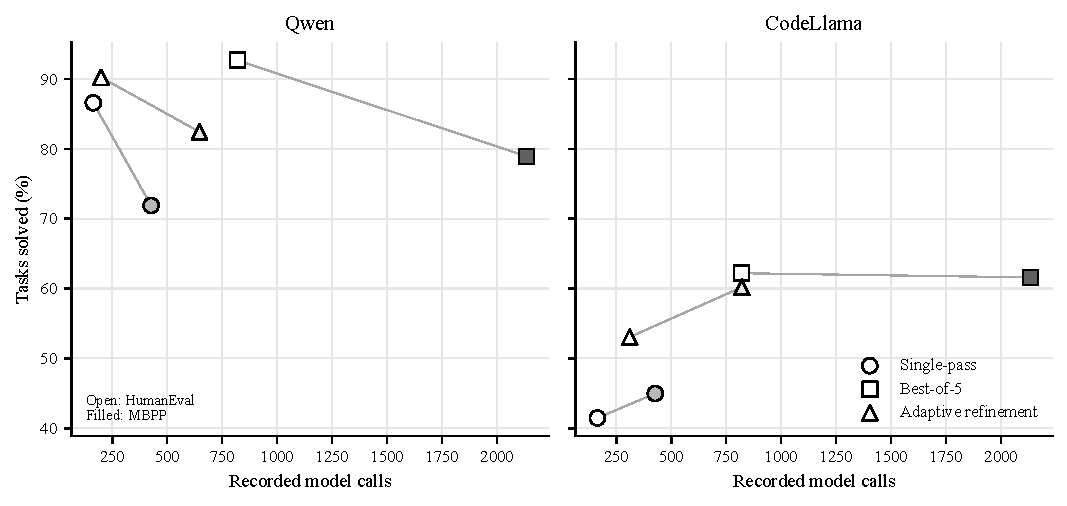
\includegraphics[width=\textwidth]{figures/figure_4_2_accuracy_calls.pdf}
    \caption{Standard-benchmark functional correctness against recorded model calls. Lines connect different benchmarks for visual identification only; they do not represent trajectories or equivalence of per-call computational cost across configurations.}
    \label{fig:accuracy-calls}
\end{figure}

\section{Harder Pro-Benchmark Results}

Table~\ref{tab:pro-results} and Figure~\ref{fig:pro-pass} report the corresponding results on HumanEval Pro and MBPP Pro. Best-of-5 attained the highest pass@1 in all four Pro conditions. Frozen 10,000-resample problem-level percentile bootstrap intervals are reported below for Best-of-5 and adaptive refinement; the paired McNemar tests remain the formal comparisons because the observations are matched by task.

\begin{table}[htbp]
    \centering
    \caption{Functional correctness, calls and adaptive-versus-Best-of-5 exact McNemar results on the Pro benchmarks.}
    \label{tab:pro-results}
    \scriptsize
    \renewcommand{\arraystretch}{1.15}
    \resizebox{\textwidth}{!}{%
    \begin{tabular}{llrrrrrr}
        \hline
        Model configuration & Benchmark & Single-pass & Best-of-5 & Adaptive & Adaptive calls & BO5 calls & Exact $p$ \\
        \hline
        Qwen bfloat16 & HumanEval Pro & 65.24\% (107/164) & 78.66\% (129/164) & 70.12\% (115/164) & 256 & 820 & 0.00257683 \\
        Qwen bfloat16 & MBPP Pro & 60.32\% (228/378) & 76.46\% (289/378) & 67.99\% (257/378) & 620 & 1,890 & $5.6141\!\times\!10^{-6}$ \\
        CodeLlama 8-bit & HumanEval Pro & 28.66\% (47/164) & 43.29\% (71/164) & 33.54\% (55/164) & 340 & 820 & 0.00700037 \\
        CodeLlama 8-bit & MBPP Pro & 37.83\% (143/378) & 54.50\% (206/378) & 46.30\% (175/378) & 718 & 1,890 & 0.000244397 \\
        \hline
    \end{tabular}}
\end{table}

\begin{figure}[htbp]
    \centering
    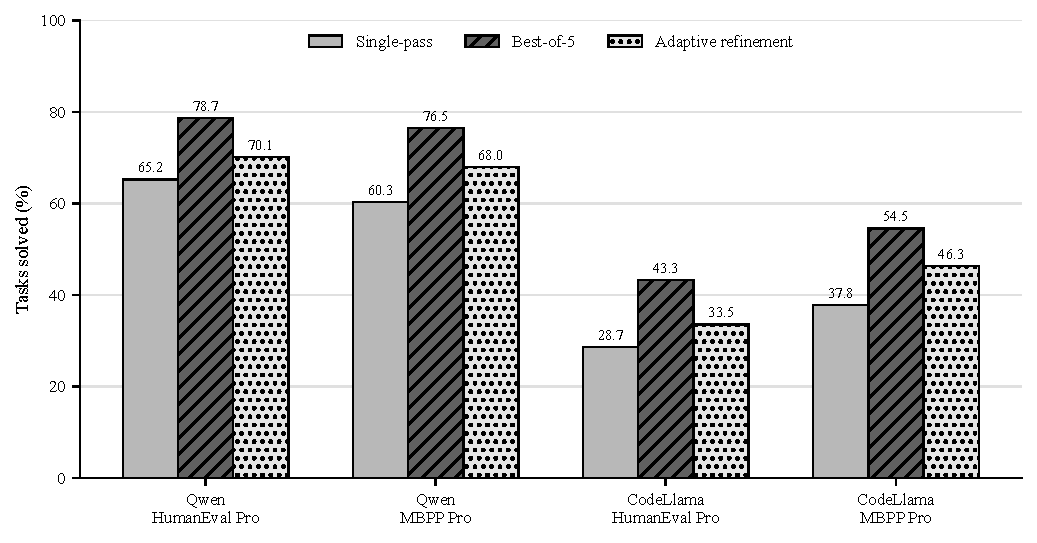
\includegraphics[width=\textwidth]{figures/figure_4_3_pro_pass_at_1.pdf}
    \caption{Problem-level pass@1 on HumanEval Pro and MBPP Pro. Best-of-5 was highest in each evaluated model--benchmark condition.}
    \label{fig:pro-pass}
\end{figure}

\subsection{HumanEval Pro}

For Qwen, single-pass solved 107 of 164 HumanEval Pro tasks (65.24\%). Best-of-5 solved 129 (78.66\%) and adaptive refinement solved 115 (70.12\%). Their bootstrap 95\% intervals were [72.56\%, 84.76\%] and [62.80\%, 76.83\%], respectively. Three tasks were adaptive-only and 17 were Best-of-5-only, giving a risk difference of $-8.54$ points, matched odds ratio 0.1765 and $p=0.00257683$.

For CodeLlama, single-pass solved 47 HumanEval Pro tasks (28.66\%). Best-of-5 solved 71 (43.29\%) and adaptive refinement solved 55 (33.54\%). Their bootstrap intervals were [35.98\%, 50.61\%] and [26.22\%, 40.85\%], respectively. The discordant counts were eight adaptive-only and 24 Best-of-5-only. The risk difference was $-9.76$ points and was statistically significant (matched odds ratio 0.3333; $p=0.00700037$).

\subsection{MBPP Pro}

For Qwen on MBPP Pro, single-pass solved 228 tasks (60.32\%). Best-of-5 solved 289 (76.46\%) and adaptive refinement solved 257 (67.99\%). Their bootstrap intervals were [72.22\%, 80.69\%] and [63.23\%, 72.75\%], respectively. Nine tasks were adaptive-only and 41 were Best-of-5-only; the risk difference was $-8.47$ points, the matched odds ratio was 0.2195, and $p=5.6141\times10^{-6}$.

CodeLlama single-pass solved 143 MBPP Pro tasks (37.83\%), Best-of-5 solved 206 (54.50\%), and adaptive refinement solved 175 (46.30\%). The Best-of-5 bootstrap interval was [49.47\%, 59.79\%], while the adaptive interval was [41.53\%, 51.32\%]. Nineteen tasks were adaptive-only and 50 were Best-of-5-only, producing a $-8.20$-point risk difference, matched odds ratio 0.3800 and $p=0.000244397$.

\subsection{Cross-Configuration Pattern on Harder Tasks}

Adaptive refinement improved over single-pass in all four Pro conditions, by between 4.88 and 8.47 percentage points. Unlike the standard benchmarks, however, it did not rank first in any Pro condition. Its deficit relative to Best-of-5 was similar across the four paired comparisons, ranging from 8.20 to 9.76 points, and each difference was statistically significant under the unadjusted condition-specific test. This common ranking occurred despite substantial differences in absolute pass@1 between the two model configurations and between the benchmark variants.

The Pro evidence therefore changes the observed strategy ranking relative to Qwen sanitised MBPP, where adaptive refinement was highest. It does not eliminate the refinement gain over a single generation: Qwen gained eight HumanEval Pro and 29 MBPP Pro tasks, while CodeLlama gained eight and 32 respectively. Rather, the five independent Best-of-5 candidates discovered more solutions than the adaptive trajectory within the same maximum generation allowance on all four harder conditions.

\section{Computational Efficiency}

Adaptive refinement used fewer model calls than Best-of-5 in every standard and Pro condition. On the standard benchmarks, calls fell from 820 to 199 for Qwen HumanEval, a reduction of 621 calls (75.7\%); from 2,135 to 647 for Qwen sanitised MBPP, a reduction of 1,488 (69.7\%); from 820 to 311 for CodeLlama HumanEval, a reduction of 509 (62.1\%); and from 2,135 to 821 for CodeLlama sanitised MBPP, a reduction of 1,314 (61.5\%). These reductions reflect adaptive termination rather than an equal realised generation count.

The same pattern held on the Pro benchmarks. Qwen adaptive refinement used 256 rather than 820 calls on HumanEval Pro (68.8\% fewer) and 620 rather than 1,890 on MBPP Pro (67.2\% fewer). CodeLlama used 340 rather than 820 calls on HumanEval Pro (58.5\% fewer) and 718 rather than 1,890 on MBPP Pro (62.0\% fewer). The call reductions therefore ranged from 58.5\% to 75.7\% across the eight authoritative conditions.

The accuracy consequence of those reductions differed by condition. Qwen sanitised MBPP combined fewer calls with a higher pass@1 than Best-of-5. CodeLlama sanitised MBPP combined 61.5\% fewer calls with a non-significant 1.41-point deficit. In contrast, both HumanEval conditions and all four Pro conditions showed lower adaptive pass@1, with the Pro deficits all statistically significant. Figure~\ref{fig:accuracy-calls} visualises the standard results, but does not imply that a Qwen call and a CodeLlama call have equal computational cost.

Authoritative prompt-token, completion-token and wall-clock totals were also recorded. They are not reproduced as a complete main-text matrix because their interpretation depends on prompt growth, generated length, model representation, hardware and run conditions. Model-call counts consequently provide a transparent measure of generation frequency, not a substitute for unmeasured FLOPs, energy or financial cost.

\section{Adaptive Convergence and Forced Continuation}

Table~\ref{tab:convergence-results} compares adaptive refinement with exactly five forced refinement iterations. Across all eight authoritative model--benchmark conditions, the adaptive and fixed procedures had identical ever-solved task sets. The paired discordant cells were therefore zero in both directions in every condition: the risk difference was zero, the Haldane--Anscombe-adjusted matched odds ratio was 1.0, and the exact McNemar $p$-value was 1.0. Forced continuation discovered no additional task beyond adaptive stopping.

\begin{table}[htbp]
    \centering
    \caption{Adaptive convergence and fixed-$k=5$ continuation. Regression denominators are fixed-run tasks solved at least once.}
    \label{tab:convergence-results}
    \scriptsize
    \renewcommand{\arraystretch}{1.15}
    \resizebox{\textwidth}{!}{%
    \begin{tabular}{llrrrrr}
        \hline
        Model configuration & Benchmark & Ever solved A/F & Fixed final & Adaptive calls & Fixed calls & Regressions \\
        \hline
        Qwen bfloat16 & HumanEval & 148/148 & 143 & 199 & 820 & 5/148 (3.4\%) \\
        Qwen bfloat16 & Sanitised MBPP & 352/352 & 334 & 647 & 2,135 & 18/352 (5.1\%) \\
        CodeLlama 8-bit & HumanEval & 87/87 & 78 & 311 & 820 & 9/87 (10.3\%) \\
        CodeLlama 8-bit & Sanitised MBPP & 257/257 & 211 & 821 & 2,135 & 46/257 (17.9\%) \\
        Qwen bfloat16 & HumanEval Pro & 115/115 & 114 & 256 & 820 & 1/115 (0.9\%) \\
        Qwen bfloat16 & MBPP Pro & 257/257 & 253 & 620 & 1,890 & 4/257 (1.6\%) \\
        CodeLlama 8-bit & HumanEval Pro & 55/55 & 54 & 340 & 820 & 1/55 (1.8\%) \\
        CodeLlama 8-bit & MBPP Pro & 175/175 & 164 & 718 & 1,890 & 11/175 (6.3\%) \\
        \hline
    \end{tabular}}
\end{table}

\begin{figure}[htbp]
    \centering
    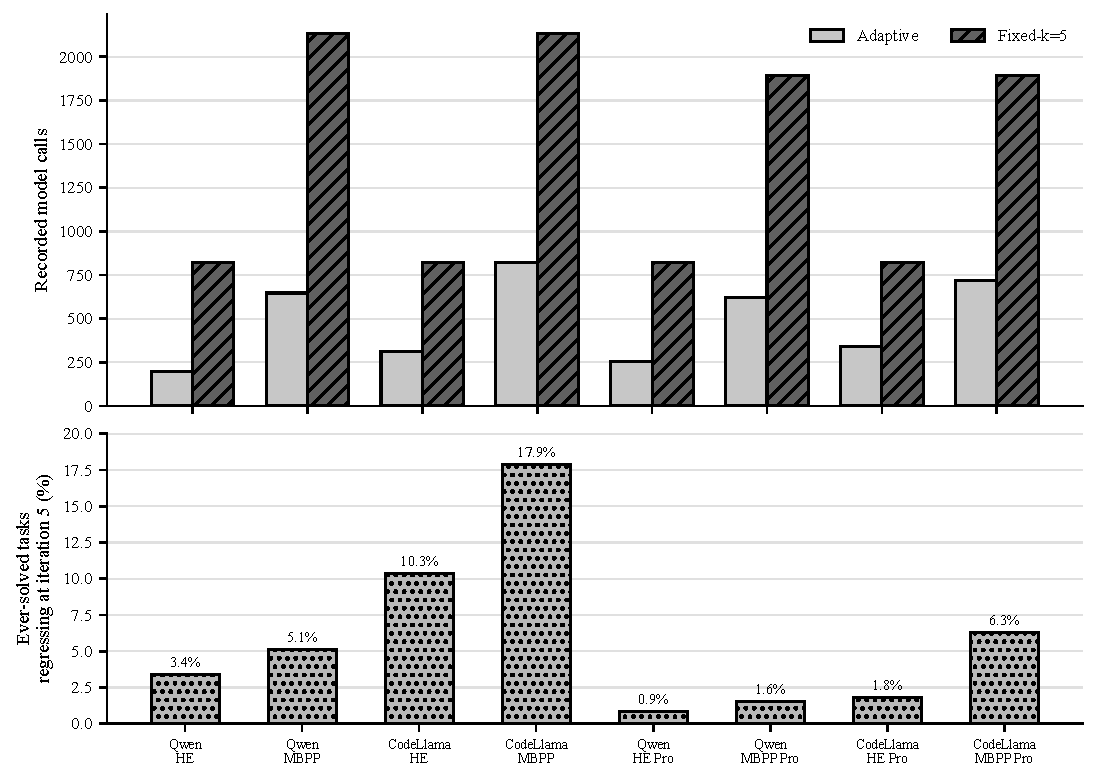
\includegraphics[width=\textwidth]{figures/figure_4_4_convergence_regressions.pdf}
    \caption{Recorded model calls under adaptive and fixed-$k=5$ refinement, with the proportion of fixed-run ever-solved tasks that failed at iteration five. A/F in Table~\ref{tab:convergence-results} denotes adaptive/fixed ever-solved counts.}
    \label{fig:convergence-regressions}
\end{figure}

The additional fixed calls were 621 and 1,488 for Qwen on the standard benchmarks, 509 and 1,314 for CodeLlama, 564 and 1,270 for Qwen on the Pro benchmarks, and 480 and 1,172 for CodeLlama. Although discovery outcomes were unchanged, final-iteration correctness decreased in every condition. The standard fixed runs regressed from ever-solved to final-failing on 5/148 Qwen HumanEval tasks (3.4\%), 18/352 Qwen MBPP tasks (5.1\%), 9/87 CodeLlama HumanEval tasks (10.3\%), and 46/257 CodeLlama MBPP tasks (17.9\%). The corresponding Pro rates were 0.9\%, 1.6\%, 1.8\% and 6.3\%.

The frozen trajectory audit identified a common recorded prompt pattern in the regression cases: after a successful execution reported ``All assertions passed.'', forced continuation nevertheless supplied a subsequent request for a corrected solution. This is reported as an observed association in the persisted trajectories. The results do not by themselves establish that this wording caused each later failure. Empirically, however, retaining the earlier passing candidate avoided the final-state losses while producing the same ever-solved outcome with fewer calls.

\section{Sensitivity Analysis}

The sensitivity analysis used the same fixed 100-task HumanEval subset for both model configurations. Figure~\ref{fig:sensitivity} presents the feedback-length and temperature results. These are fixed-seed descriptive comparisons; no frozen sensitivity confidence intervals or paired statistical outputs are available.

\begin{figure}[htbp]
    \centering
    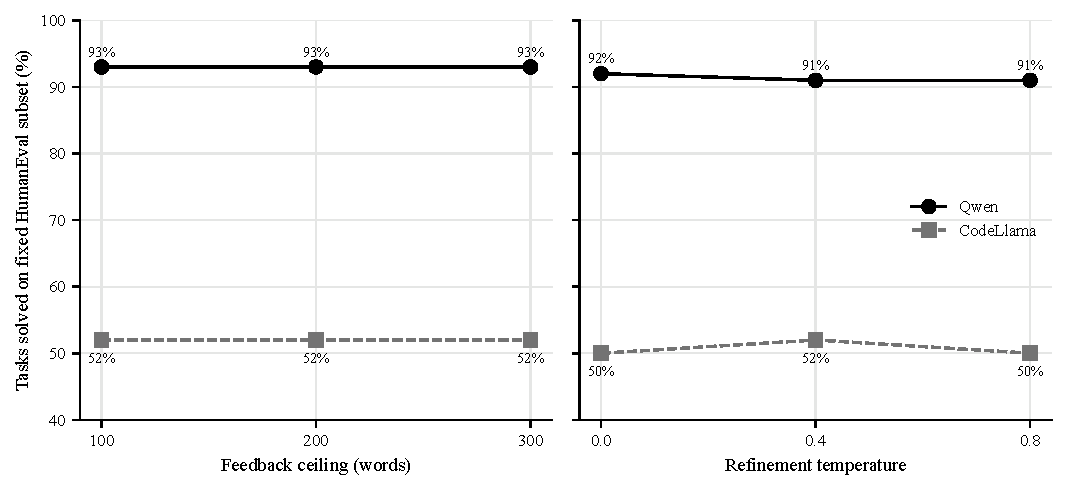
\includegraphics[width=\textwidth]{figures/figure_4_5_sensitivity.pdf}
    \caption{Adaptive-refinement sensitivity on the fixed 100-task HumanEval subset. The left panel varies the feedback ceiling at temperature 0.2; the right varies temperature without the explicit feedback-word ceiling.}
    \label{fig:sensitivity}
\end{figure}

\subsection{Feedback-Length Sensitivity}

Qwen solved 93 of 100 tasks under each of the 100-, 200- and 300-word feedback ceilings, using 116 calls in every condition. CodeLlama solved 52 of 100 tasks under each ceiling and used 187 calls in every condition. Within each model, the three settings produced identical problem-level pass/fail vectors, not merely equal aggregate counts. The corresponding prompt- and completion-token totals were identical within each model because none of the observed rendered feedback exceeded the lowest 100-word ceiling.

The result is bounded to the three evaluated word ceilings, this fixed HumanEval subset and these two model configurations. It establishes no observed sensitivity within that range; it does not establish that feedback length is irrelevant under shorter ceilings, different feedback contents, other tasks or other inference configurations.

\subsection{Temperature Sensitivity}

For Qwen, temperature 0.0 solved 92/100 tasks and temperatures 0.4 and 0.8 each solved 91/100. All three conditions used 122 calls. For CodeLlama, temperatures 0.0, 0.4 and 0.8 solved 50, 52 and 50 tasks respectively. The first two used 190 calls, while temperature 0.8 used 198. No monotonic accuracy pattern was observed across the three temperature settings for either configuration.

The numerical spread was at most two tasks within a model, but one fixed-seed run represented each condition. These results therefore describe sensitivity under the specified protocol rather than run-to-run variability or a general temperature optimum. Temperature 0.4 matched the 52/100 CodeLlama reference-temperature outcome, whereas both the lower and higher evaluated settings solved 50 tasks.

\section{Failure and Behavioural Analysis}

The frozen failure taxonomy examined a stratified set of 50 terminal refinement failures. Of these, 25 cases (50\%) were classified as persistent despite correct feedback, eight (16\%) as receiving insufficient feedback, and 17 (34\%) as following a fundamentally wrong approach. These mechanism labels distinguish failures in which an actionable diagnostic was not used from cases in which the available diagnostic did not expose the decisive defect, and from trajectories that did not approach the required algorithm.

Logic errors accounted for 35/50 cases (70\%), edge-case failures for 9/50 (18\%), and runtime failures for 6/50 (12\%); no sampled terminal case was classified as syntax or timeout. Terminal convergence was attributed to oscillation in 32 cases (64\%), stagnation in 14 (28\%), and maximum iterations in four (8\%). The dominance of logic failures and oscillation describes this selected failure sample and is not a population-weighted estimate for all benchmark tasks.

A separate blinded cross-model coding check compared the original Codex labels with independent Claude labels on 12 stratified cases. Agreement was 12/12 for both terminal error category and failure mechanism, with Cohen's $\kappa=1.0$ on both axes. This is a small AI-rater consistency check rather than a human inter-rater reliability study, and both raters assessed the same recorded evidence. It supports the internal reproducibility of the applied labels on those cases but does not independently validate every label or generalise beyond the sample.

The behavioural evidence complements the aggregate results by showing that terminal non-success did not represent one uniform failure mode. Half of the audited cases persisted despite feedback classified as correct, while one sixth were assigned to insufficient feedback and approximately one third retained a fundamentally wrong approach. Mechanistic explanations and implications for improved feedback design are reserved for Chapter~5.

\section{Chapter Summary}

Adaptive refinement improved over single-pass in all eight core model--benchmark conditions. Its position relative to generation-budget-matched Best-of-5 varied on the standard benchmarks: it was four tasks lower for Qwen HumanEval, 15 higher for Qwen sanitised MBPP, 15 lower for CodeLlama HumanEval and six lower for CodeLlama sanitised MBPP. The paired difference favoured adaptive refinement significantly only for Qwen MBPP; it favoured Best-of-5 significantly for CodeLlama HumanEval, while the other two standard differences were not statistically significant.

On the harder Pro benchmarks, Best-of-5 was highest in all four conditions. Adaptive refinement remained above single-pass, but trailed Best-of-5 by 8.20--9.76 percentage points, with each paired difference statistically significant under the unadjusted condition-specific test. Across the complete standard and Pro matrix, adaptive refinement used 58.5--75.7\% fewer recorded model calls than Best-of-5.

The convergence ablation produced the most uniform result: adaptive and fixed-$k=5$ refinement discovered exactly the same tasks in all eight conditions. Fixed continuation used 480--1,488 additional calls and produced final-state regressions in every condition, without discovering an additional task. Feedback-length ceilings of 100, 200 and 300 words produced identical outcome vectors within each model on the sensitivity subset, while the evaluated temperature changes produced only small, non-monotonic aggregate differences. Finally, the 50-case failure analysis was dominated by logic errors and oscillation, with multiple distinct recorded failure mechanisms. These findings provide the empirical basis for the interpretation and limitations developed in Chapter~5.

\chapter{Discussion}

\section{Overview}

\section{RQ1: Effectiveness of Execution Feedback}

\section{RQ2: Refinement versus Independent Sampling}

\section{RQ3: Adaptive Convergence}

\section{RQ4: Robustness Across Models and Benchmarks}

\section{Relationship to Prior Research}

\section{Implications}

\section{Threats to Validity and Limitations}
\chapter{Conclusion and Future Work}

\section{Summary of the Research}

\section{Answers to the Research Questions}

\section{Research Contributions}

\section{Limitations}

\section{Future Work}

\section{Final Conclusion}

%%%%%%%%%%%%%%%%%%%ETC%%%%%%%%%%%%%%%%%%%%%%
\addcontentsline{toc}{chapter}{Bibliography}
\bibliographystyle{./style/myabbrvnat}
\bibliography{./references/thesisbib}


%\addcontentsline{toc}{chapter}{List of Publications} % If you have published anything during your research
%\include{./chapters/listofpapers}

%\pagestyle{fancyplain}
\clearpage
\addcontentsline{toc}{chapter}{Appendix}
\chapter*{Appendix}
You may have one or more appendices containing detail, bulky or reference material that is relevant though supplementary to the main text: perhaps additional specifications, tables or diagrams that would distract the reader if placed in the main part of the dissertation. Make sure that you place appropriate cross-references in the main text to direct the reader to the relevant appendices.
Again you should discuss with your supervisor what appendices are appropriate for this work.

Note that you should {\bf not} include your program listings as an appendix or appendices. You should submit one copy of such bulky text as a separate item, perhaps on a disk.




\end{document}
%\end{normalsize}
